\section{Ontology Matching}
\section{Experiment}
\label{sec:experiment}
Because we are interested in understanding the property of the Pareto front obtained by our method, we conducted a series of experiments to highlight tradeoffs of the objectives functions. First, to illustrate the proposed method is indeed capable of determining matching between numeric-typed attributes and clusters, we synthesized a dataset simulating some extreme conditions under which previous methods are ineffective. Also, from the results obtained on the synthetic dataset, we empirically study tradeoffs between the two objective functions. Then, to evaluate the scalability of the method, we carry out a series of tests on a set of data with varied sizes. Finally, encouraged by these results, we applied our methods to actual neuroscience ERP (event-related potentials) data to highlight the applicability of our method to the neuroscience domain.

\subsection{Synthetic Dataset}
\label{sec:syn_exp}
\subsubsection{Data Generation:}
In the synthetic dataset, we generated values for each attribute in such a way that each attribute can be divided into several clusters, and each cluster corresponds to a Gaussian distribution with different mean and standard deviation, but the overall mean and standard deviation of values from all clusters in one attribute are made very close to those in other attributes. For example, Figure~\ref{fig:syndata} illustrates the value distributions of three attributes ($a_1, a_2,$ and $a_3$) from one dataset and their corresponding counterparts ($a_1', a_2',$ and $a_3'$) from another. It shows that the overall means and standard deviations for these six attributes are almost indistinguishable, and their ranges are similar as well. Previous methods using these whole-attribute-wise quantities as statistical characterization of attributes would have a hard time determining the matchings. However, as mentioned above and illustrated in the figure, the individual distributions underlying clusters in these attributes are distinct and, by using the segmented statistical characterization of attributes, the difference is significant enough to differentiate and identify matchings between attributes.

\begin{figure*}[tbh]
\begin{center}
\begin{tabular}{ccc}
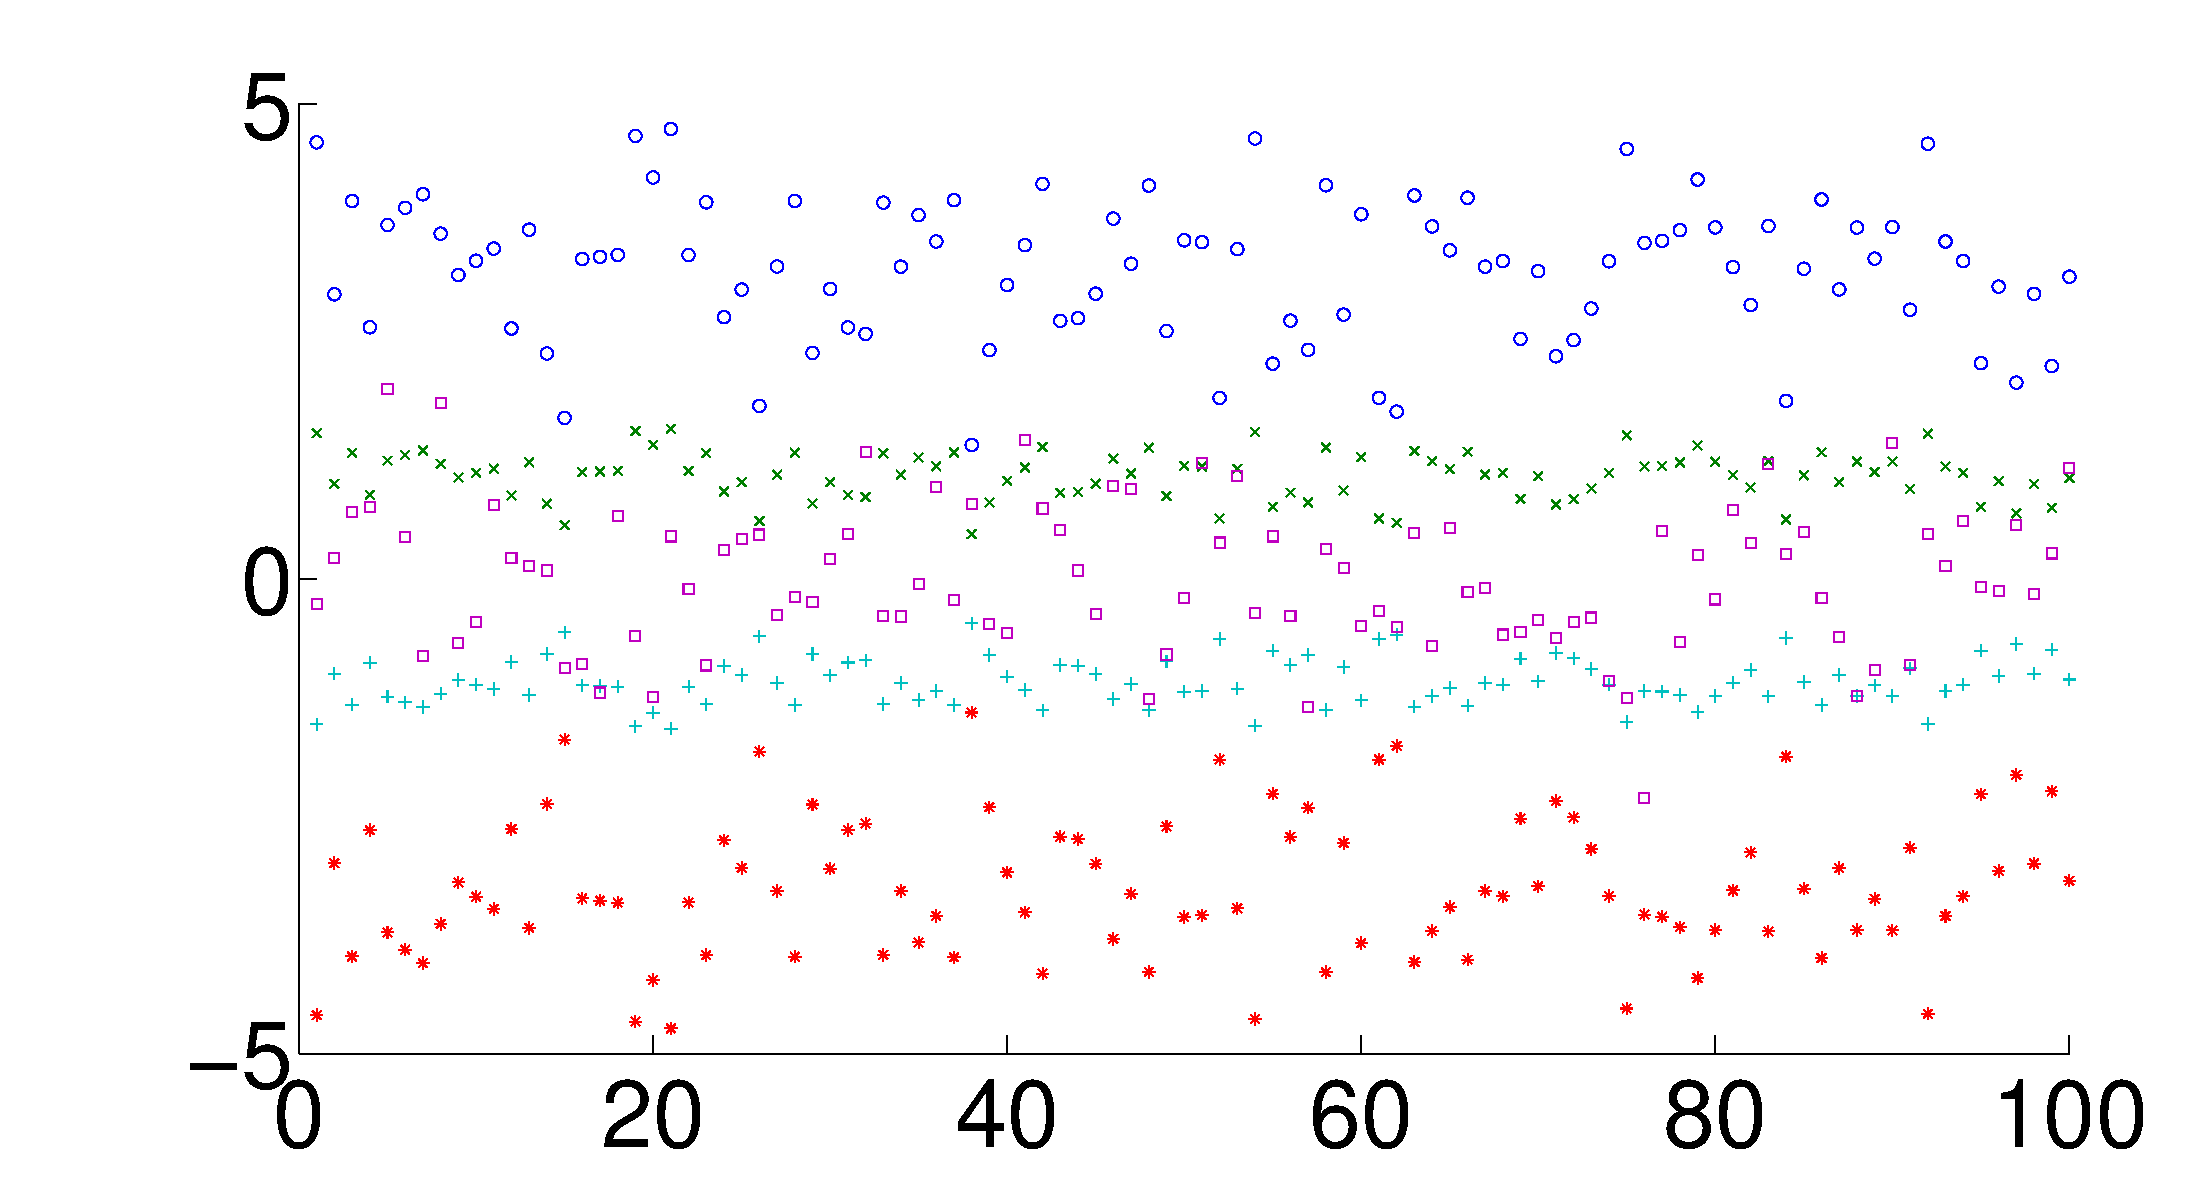
\includegraphics[scale=0.14]{fig/clusters.eps} &
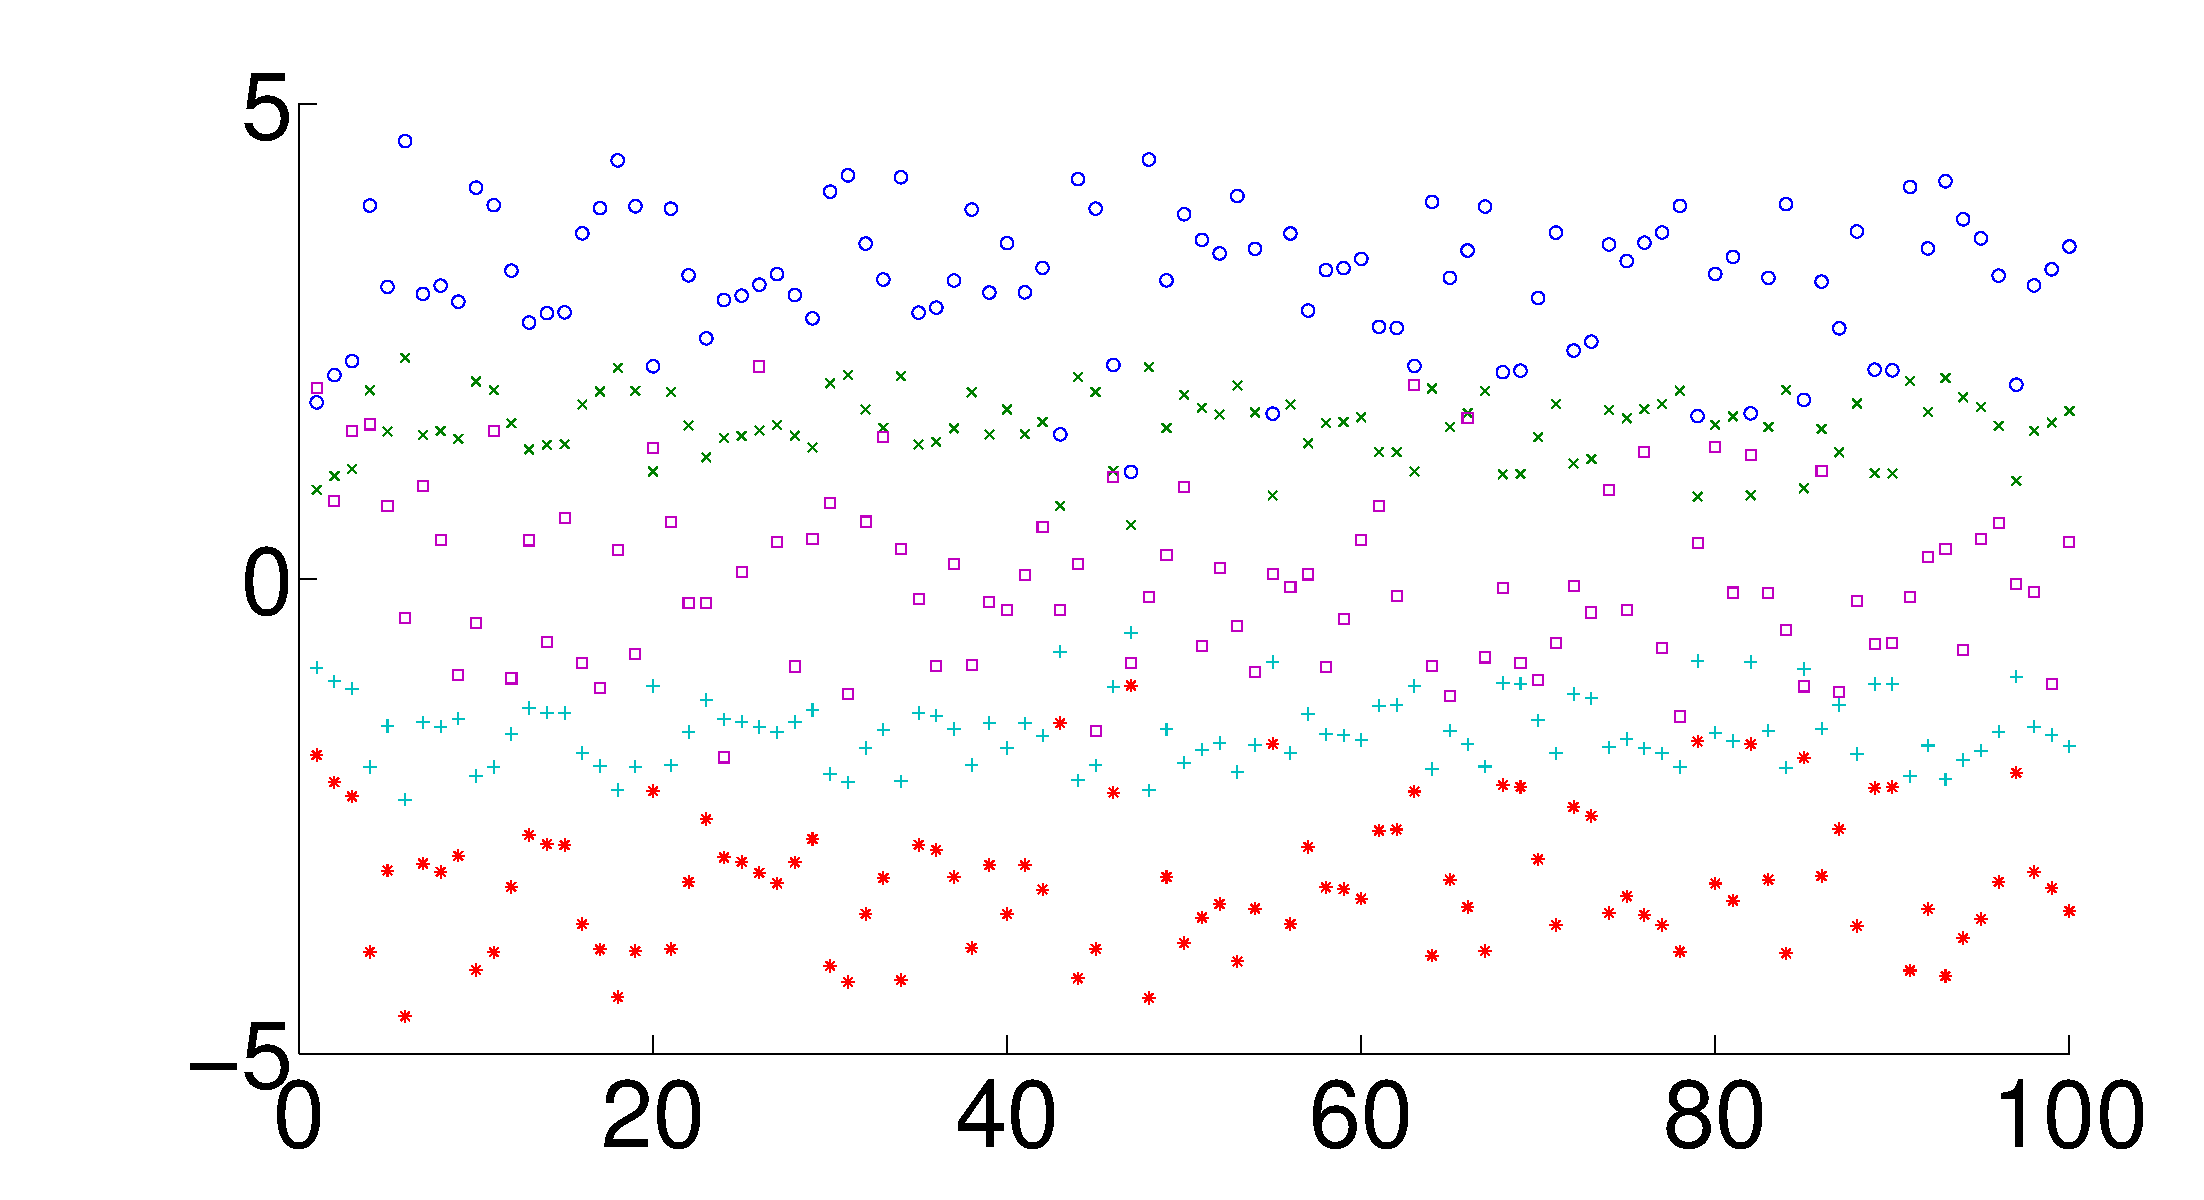
\includegraphics[scale=0.14]{fig/clusters4.eps} &
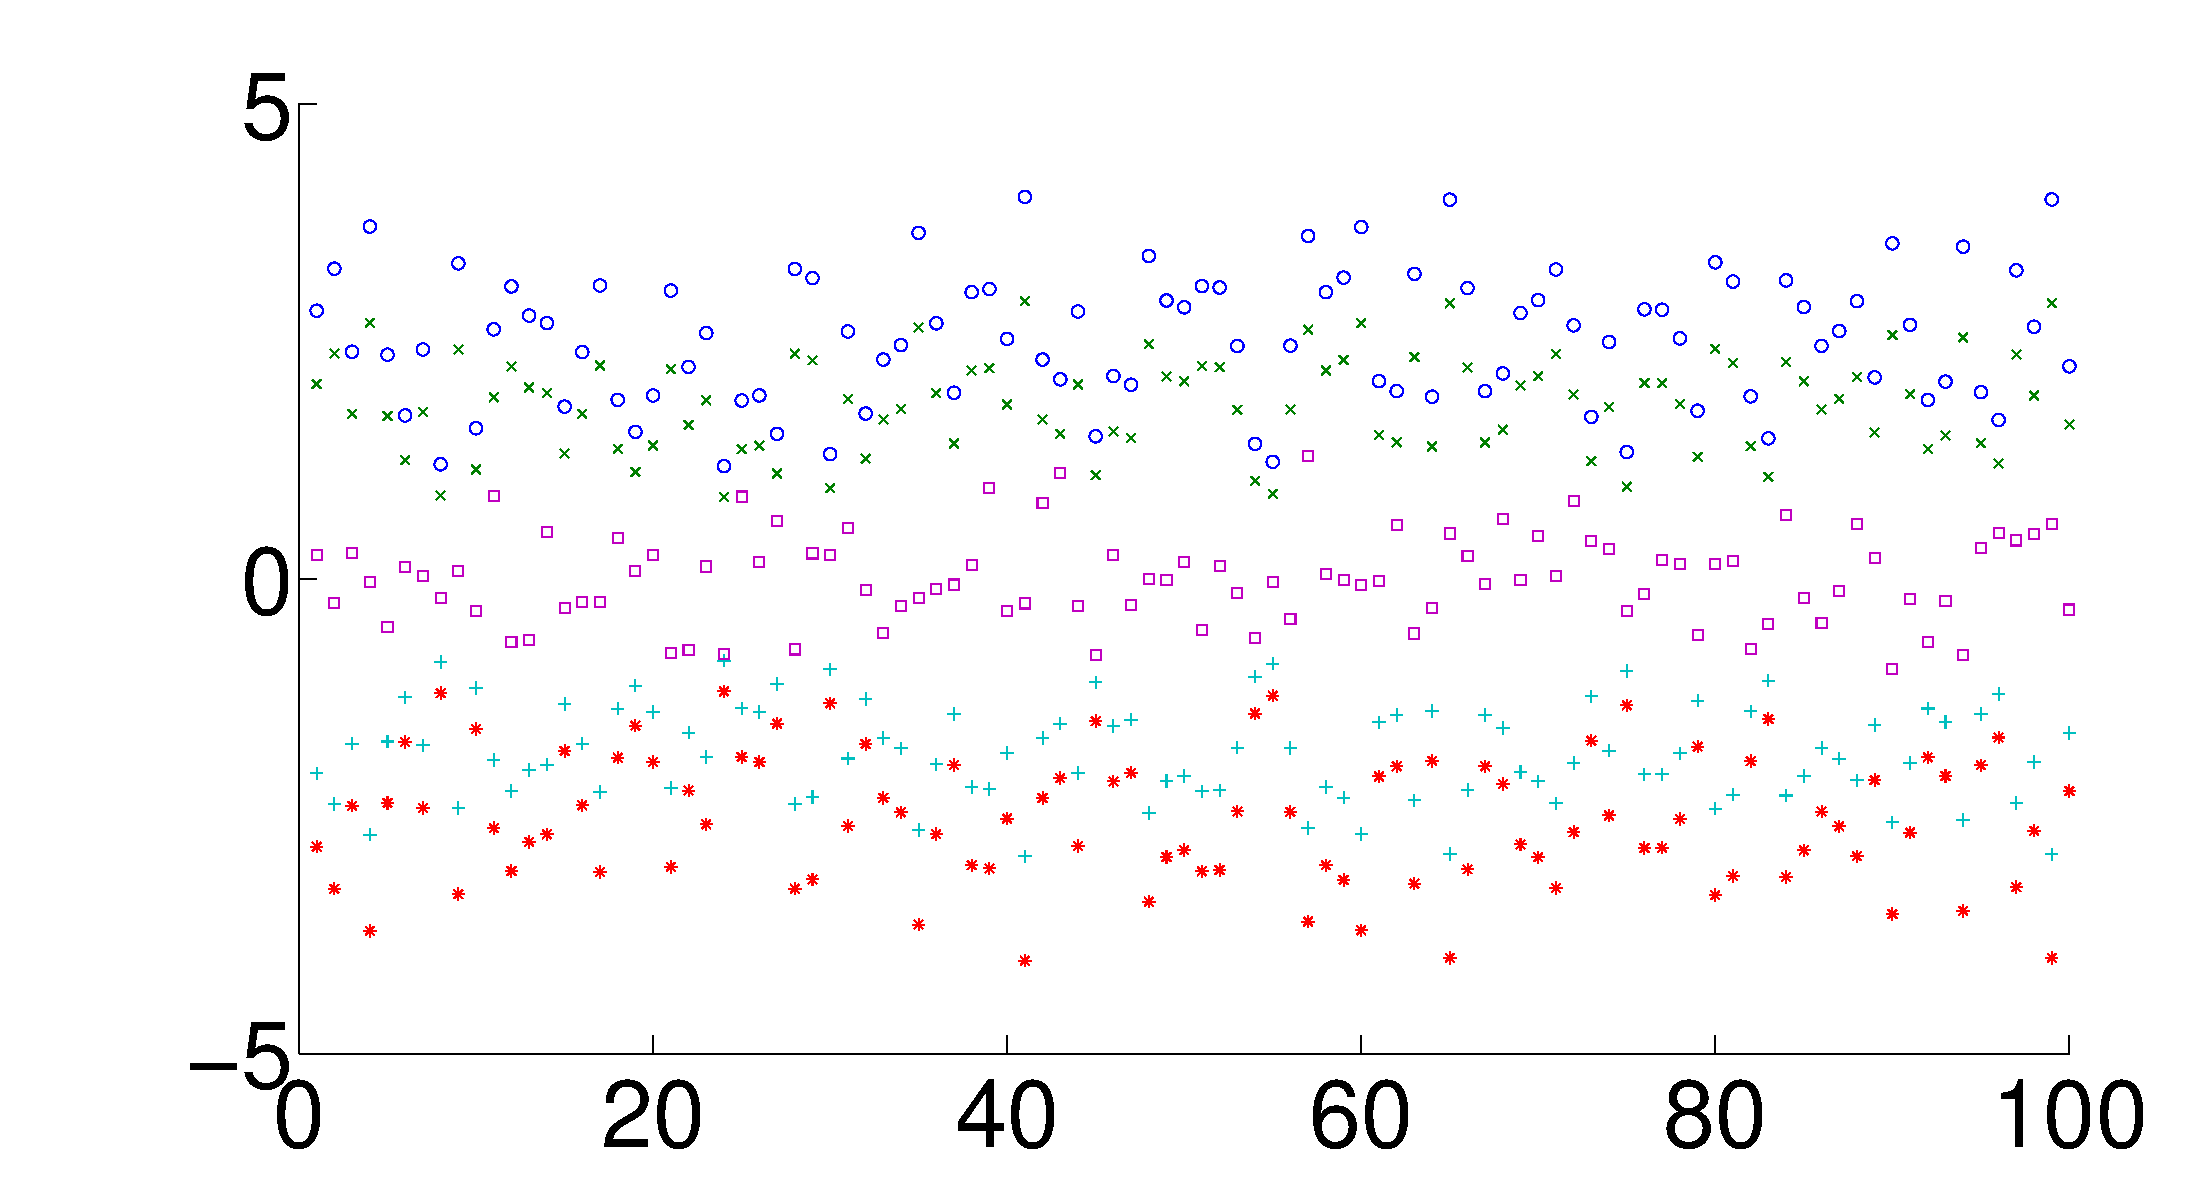
\includegraphics[scale=0.14]{fig/clusters3.eps} \\
$a_1$ --- range: [-4.74, 4.74] & $a_3$ --- range: [-4.61, 4.61] & $a_2$ --- range: [-4.02, 4.02] \\
$\mu$: 0, $\sigma$:2.26 &$\mu$: 0, $\sigma$:2.30 & $\mu$: 0, $\sigma$:2.18 \\
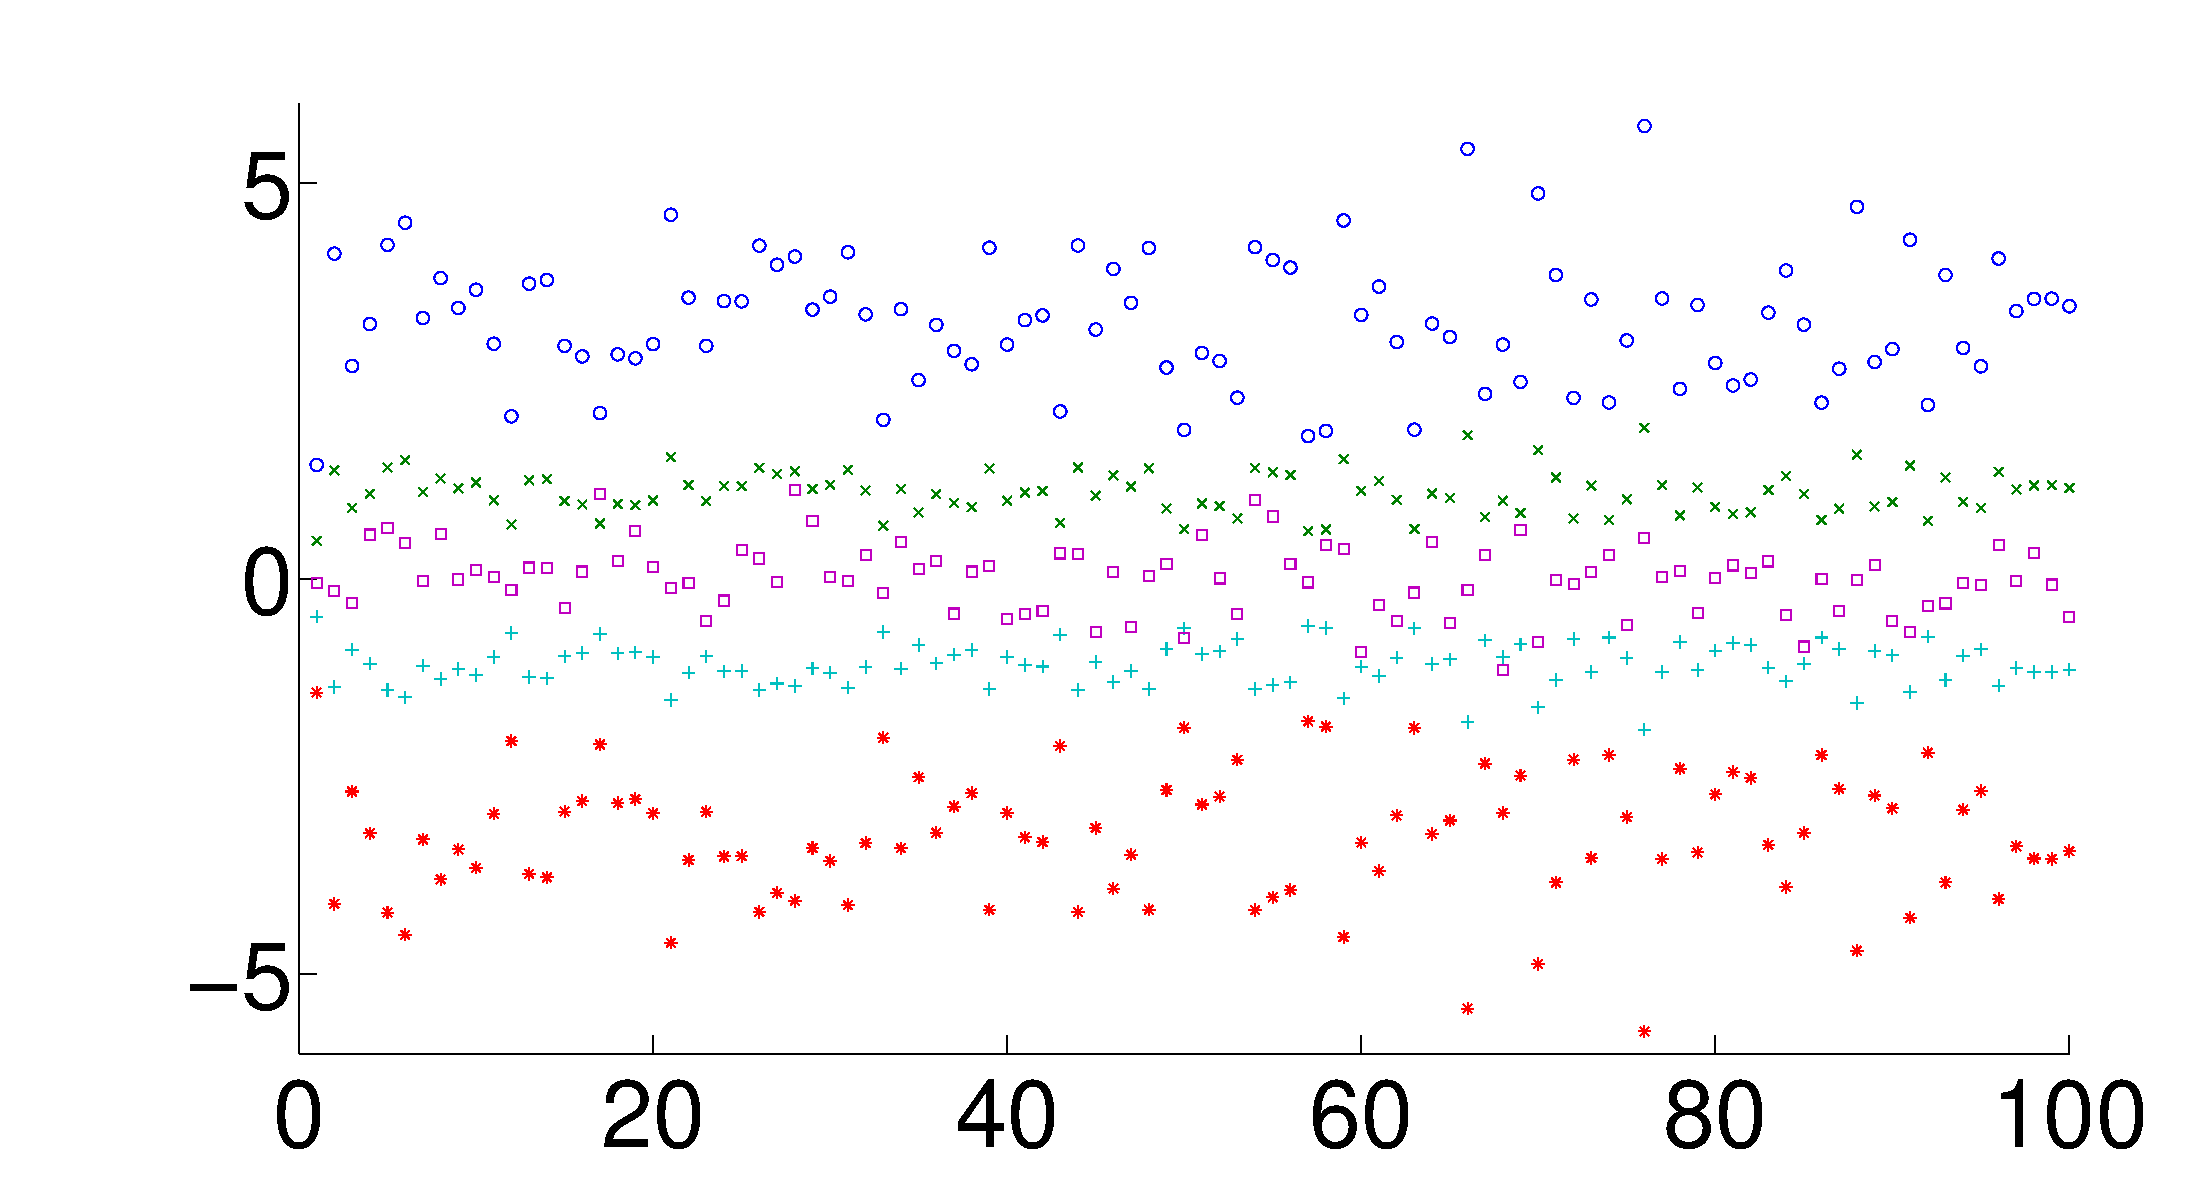
\includegraphics[scale=0.14]{fig/clusters21.eps} &
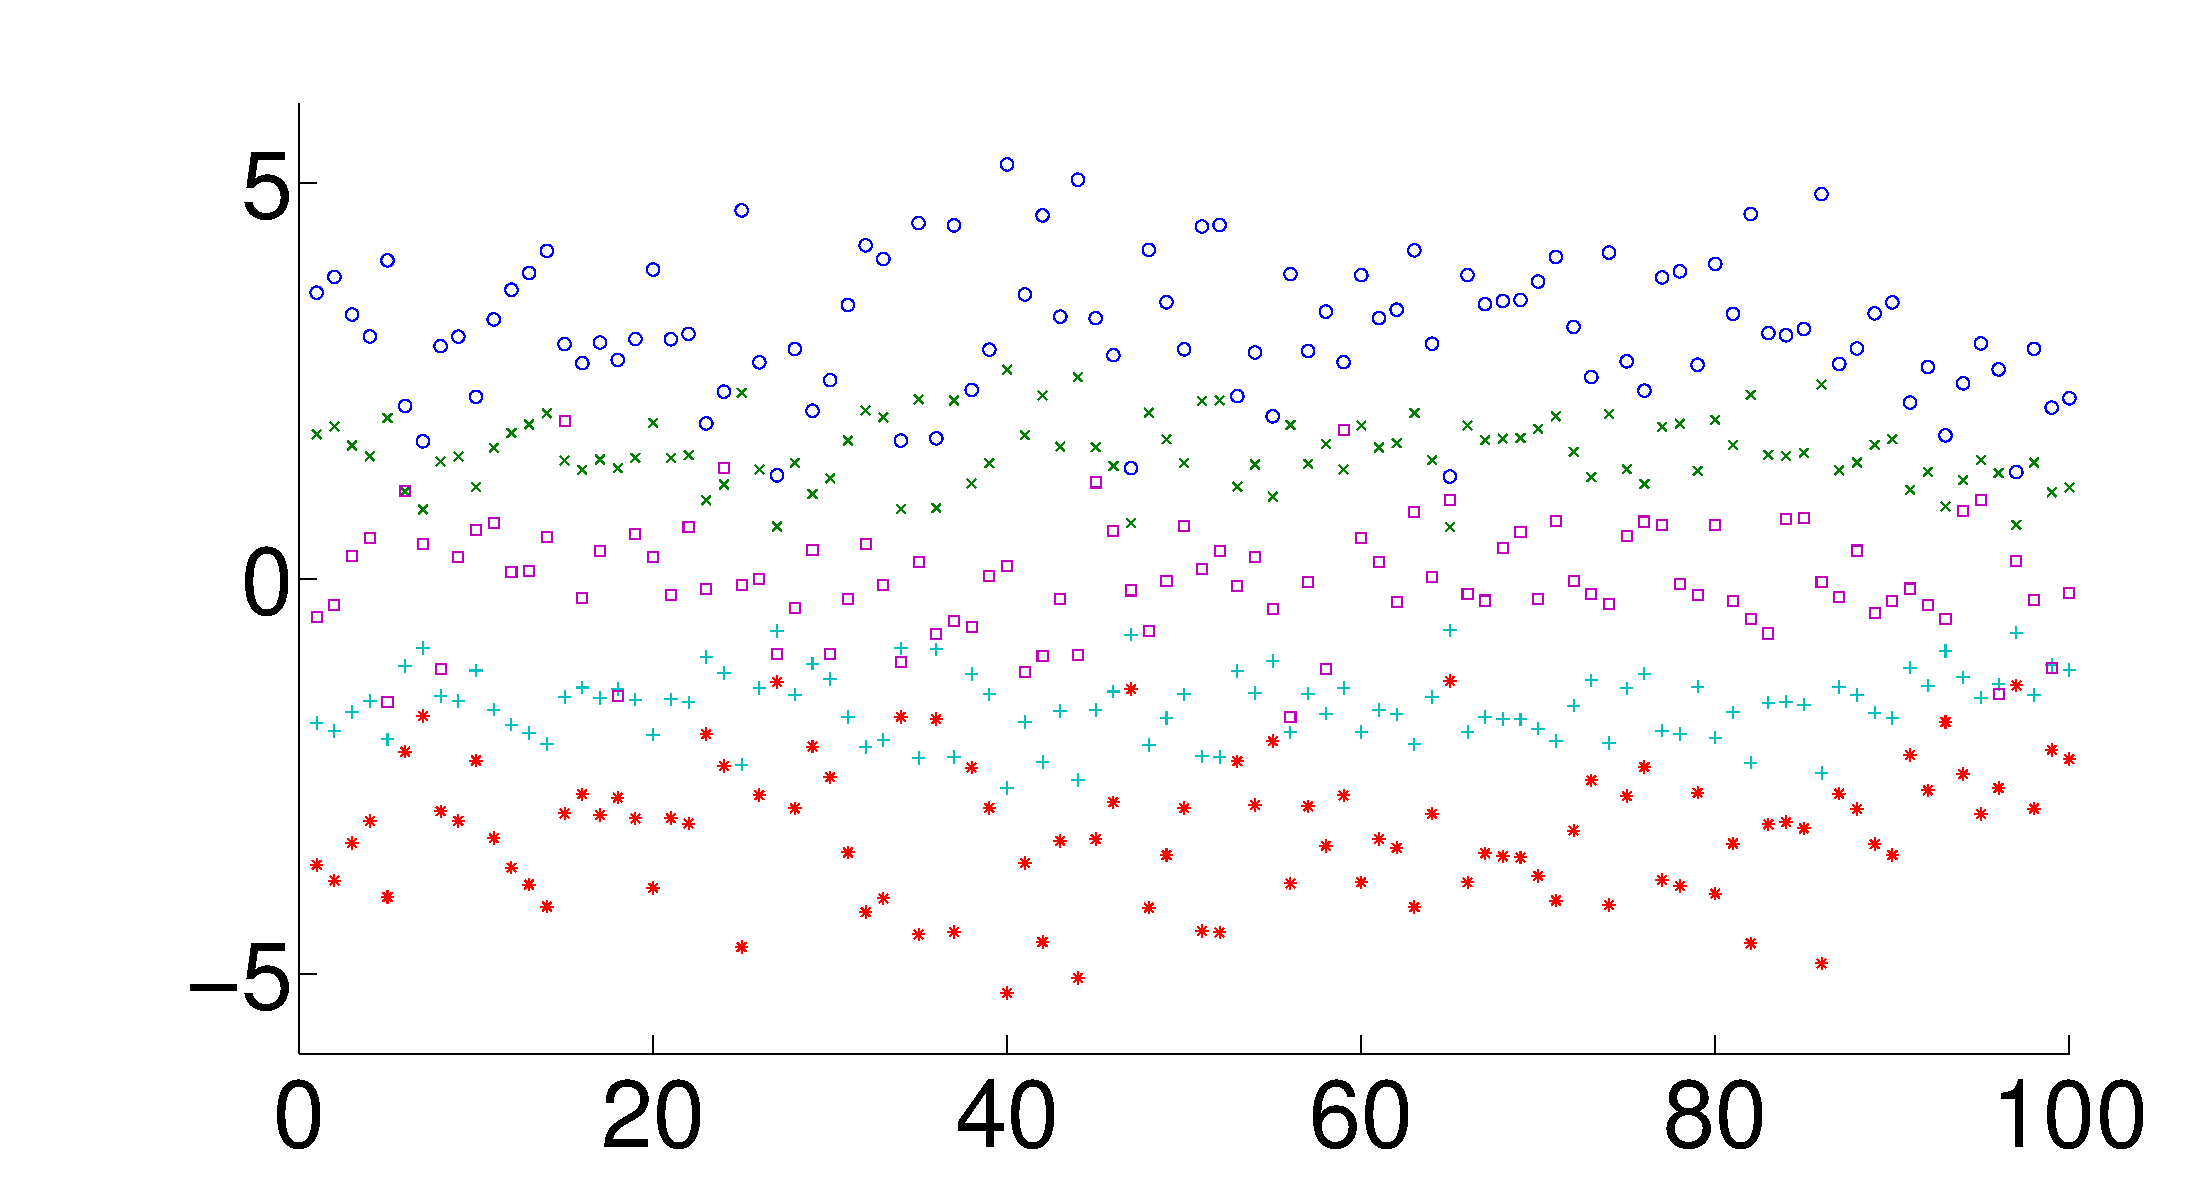
\includegraphics[scale=0.14]{fig/clusters23.eps} &
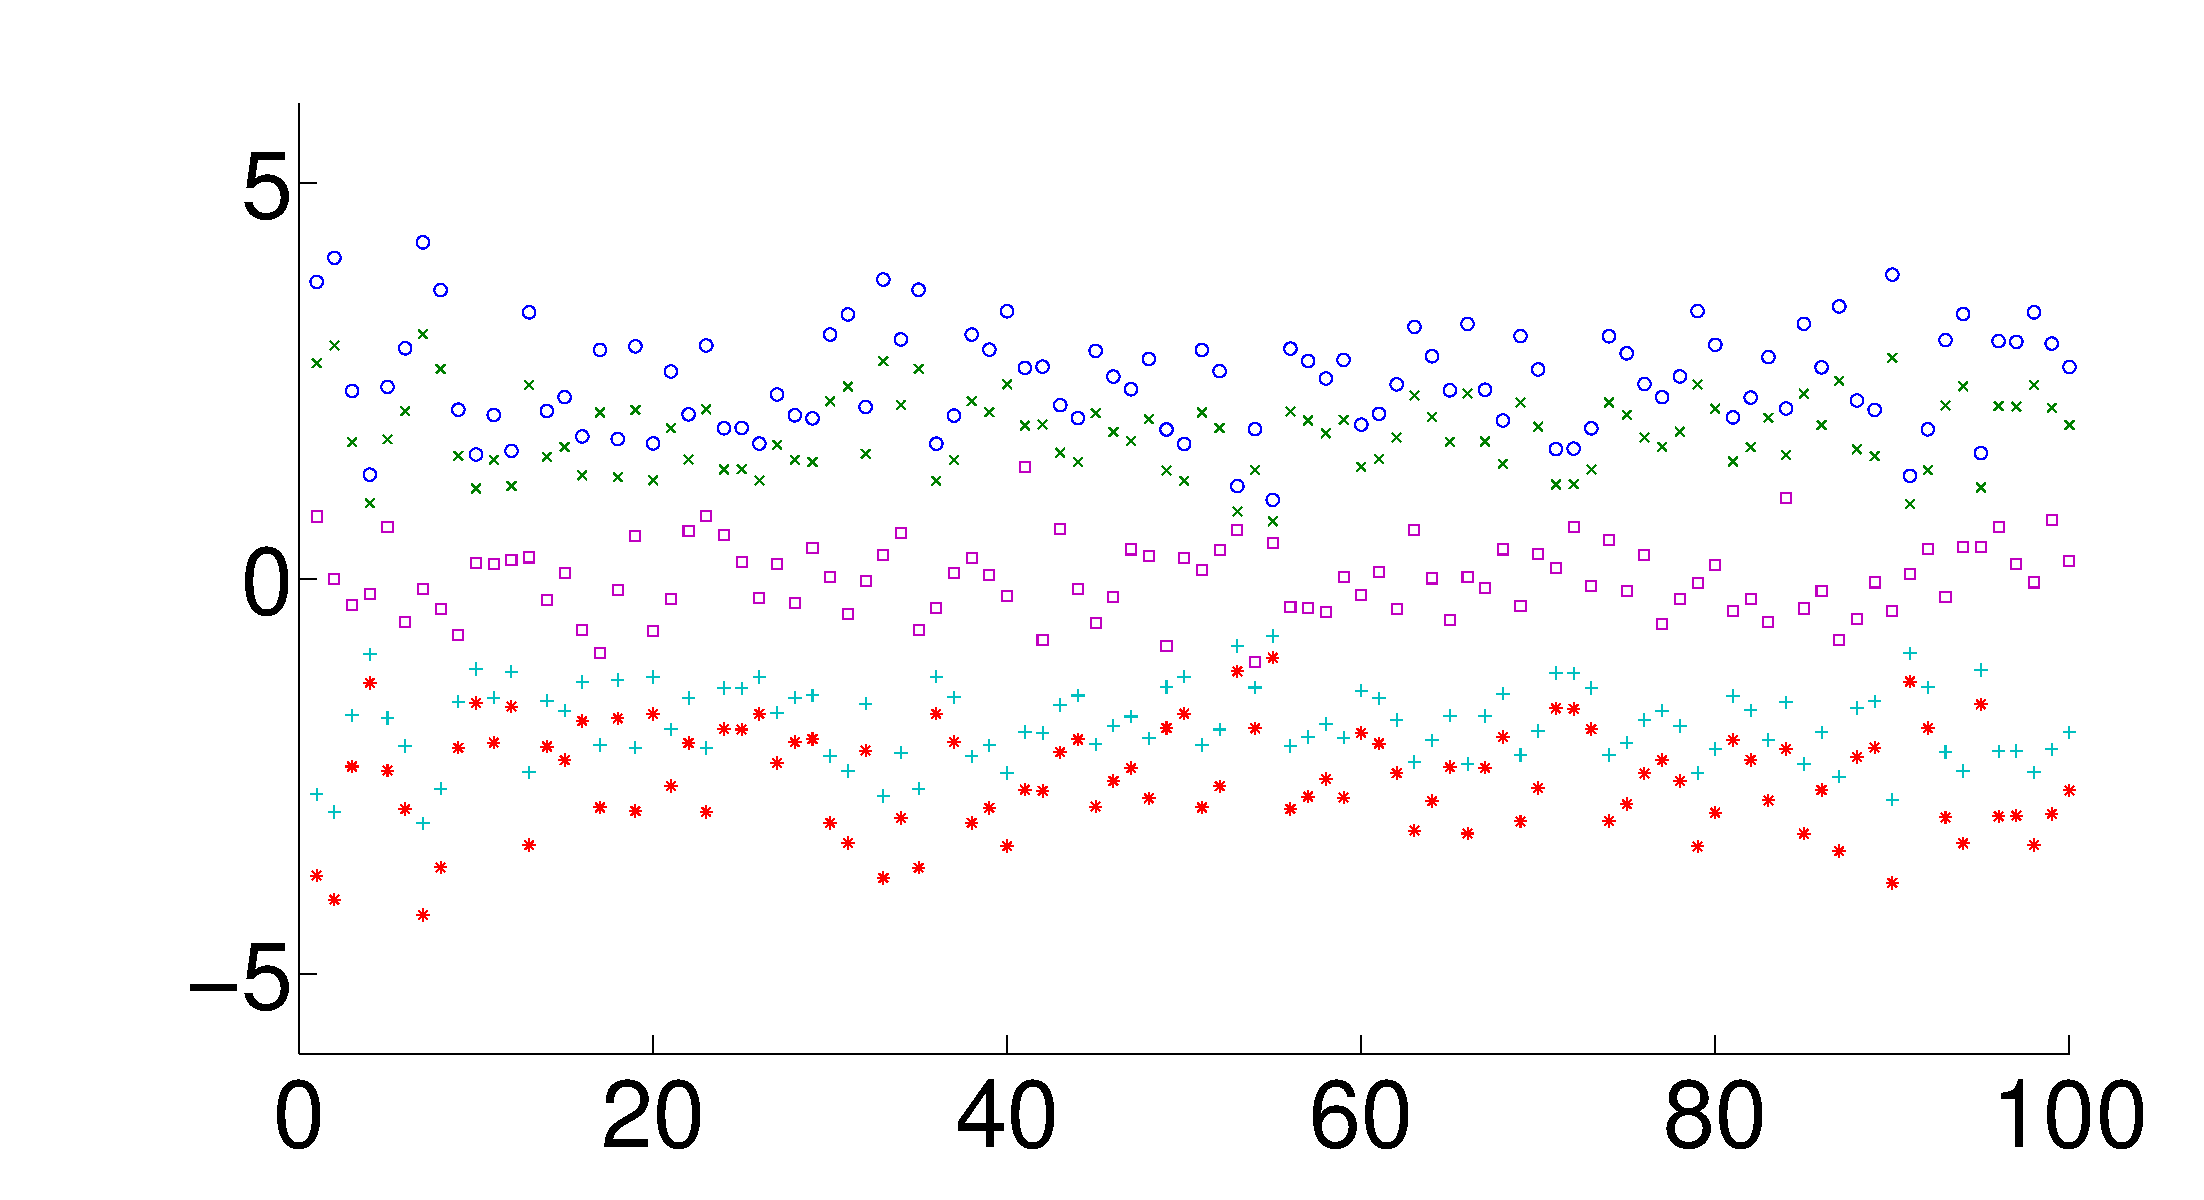
\includegraphics[scale=0.14]{fig/clusters22.eps} \\
$a_1'$ --- range: [-5.72, 5.72] & $a_3'$ --- range: [-5.24, 5.24] & $a_2'$ --- range: [-4.25, 4.25] \\
$\mu$: 0, $\sigma$:2.20 & $\mu$: 0, $\sigma$:2.35 & $\mu$: 0, $\sigma$:2.15 \\
\end{tabular}
\end{center}
\caption{\label{fig:syndata} Scatter plots of data instances from three sample attributes in one synthetic dataset (upper frame) and those of their corresponding attributes from another (lower frame) are illustrated to show their respective value distributions.}
\end{figure*}

\subsubsection{Results:}
Figure~\ref{fig:syn_pareto} illustrates the Pareto front obtained from matching two synthetic datasets, each having 20 attributes and 5 clusters. Most notably, the gold standard results for both attribute matching and cluster matching are obtained from the left-most point on the Pareto front. In other words, given the decision variables ($X$) corresponding to that point, we obtained 100\% correct matching results. We further observed that in our subsequent tests on other synthetic datasets with varied number of attributes and clusters, the derived Pareto fronts all contain gold standard result, and the point corresponding to the gold standard can always be found towards the minimum end of $f_a$. Given this, we propose the following method to reduce the Pareto-optimal set to a single point corresponding to the most favored choice ($X^*$) in the decision space. The idea is to find the decision with the minimum weighted sum of objective values in the obtained Pareto-optimal set, i.e., $X^*=\stackbin[X]{}{\argmin}~\big[\alpha f_a(X)+\beta f_c(X)\big]$, where $\alpha$ and $\beta$ are weights. We first conducted preliminary experiments to determine the best values for $\alpha$ and $\beta$ (0.8 and 0.2 respectively) and used them in all subsequent experiments. This method works markedly well on the synthetic datasets. For all the tests described in Table~\ref{tbl:scale}, 100\% correct results for both attribute and cluster matchings are obtained (hence we omit the precision in the table).
\begin{figure}[tb]
\begin{center}
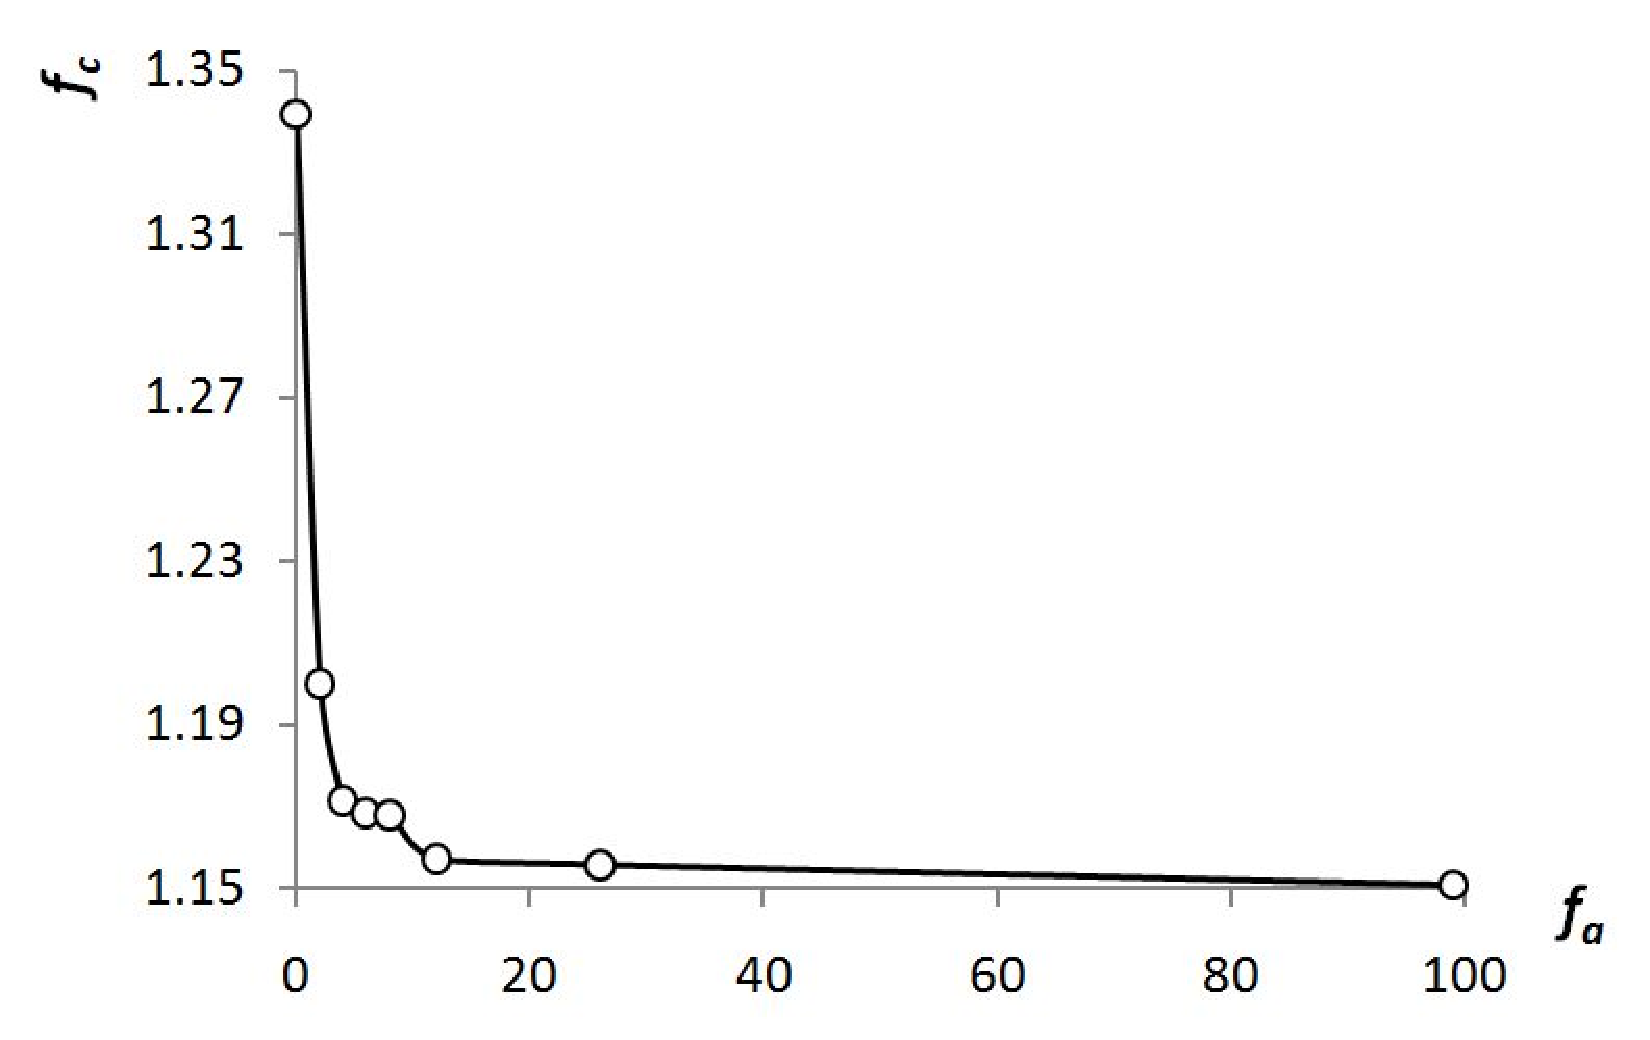
\includegraphics[width=0.6\textwidth]{fig/syn_pareto.eps}
\end{center}
\caption{\label{fig:syn_pareto} An example Pareto front obtained from matching two synthetic datasets with 20 attributes and 5 clusters.}
\end{figure}

\subsubsection{Running Time:}
We systematically altered the number of attributes and clusters present in the data and conducted a series of tests to show the scalability of the proposed method. The running time under different configurations is reported in Table~\ref{tbl:scale}. The time is calculated by averaging over 5 runs of each test (on a 2.53GHz dual-core CPU with 4 gigabytes memory), each run having 1000 iterations in the simulated annealing process. The main computationally expensive part of the annealing process is the generation of new candidate solution phase (function $G$) in which an assignment problem is solved using the Hungarian method. The complexity of the Hungarian method is cubic and is already the most efficient algorithm for solving the assignment problem (a brute force algorithm has a factorial complexity). Fortunately, rarely is the case that the number of attributes or clusters is large in real-world scenarios where the proposed technique is needed. For reasonable configurations in most practical applications, the computation time is within a tractable range as shown in table~\ref{tbl:scale}.
\begin{table}[tbh]
\begin{center}
\begin{tabular}{r|r|r}
\hline
\# attributes & \# clusters & time (sec)\\
\hline
5   &   20  &   0.28\\
20  &   20  &   1.81\\
20  &   40  &   7.04\\
20  &   60  &   17.80\\
40  &   20  &   4.66\\
40  &   40  &   11.74\\
40  &   60  &   25.93\\
60  &   20  &   10.95\\
60  &   40  &   20.70\\
60  &   60  &   37.35\\
100 &   100 &   172.23\\
\hline
\end{tabular}
\end{center}
\caption{\label{tbl:scale} Running time of the annealing process on synthetic datasets with varied configurations of attribute and cluster sizes. The time is obtained by averaging over results of 5 runs of each test.}
\end{table}

\subsection{Neuroscience Dataset}
\subsubsection{Data Acquisition:}
%The difficulty is especially pronounced in many scientific domains where there have been an increasing interest in nationwide and worldwide inter-institute collaboration. An example of such collaborative project is research in experimental event-related brain potential (ERP) analysis carried out at the NEMO (Neural Electromagnetic Ontologies) consortium laboratories. The heterogeneity among participating groups hinders meaningful meta-analysis despite the large number of studies in the field.

To address the problems of attribute and cluster matching in a real-world neuroscience application, we used a set of realistic simulated ERP (event-related potentials) datasets, which were designed to support evaluation of ERP analysis methods~\cite{FrishkoffEtal07}. The datasets were specifically designed to simulate heterogeneous data from different groups of subjects under different conditions (via distinct simulated brain activities), as well as distinct measurement methods (spatial and temporal metrics) and distinct patterns (reflecting two different pattern decomposition techniques). Real ERP data arise from superposition of latent scalp-surface electrophysiological patterns, each reflecting the activity of a distinct cortical network that cannot be reconstructed from the scalp-measured data with any certainty. Thus, real ERP data are not appropriate for evaluation of ERP pattern mapping. By contrast, simulated ERP data are derived from known source patterns and therefore provide the necessary gold standard for evaluation of our proposed methods.

The raw data for this study consist of 80 simulated event-related potentials (ERPs), in which each ERP comprises simulated measurement data for a particular subject ($n$ = 40). The 40 simulated subjects are randomly divided into two 20-subject groups, SG1 and SG2, each containing 40 ERPs (20 subjects in 2 experimental conditions). Each ERP consists of a superposition of 5 latent varying spatiotemporal patterns. These patterns were extracted from the two datasets, SG1 and SG2, using two techniques: temporal Principal Components Analysis (tPCA) and spatial Independent Components Analysis (sICA), two data decomposition techniques widely used in ERP research~\cite{Dien2010}. To quantify the spatiotemporal characteristics of the extracted patterns, two alternative metric sets, m1 and m2, were applied to the two tPCA and the two sICA derived datasets. For a complete explanation of these alternative metrics, please see Appendix in~\cite{FrishkoffEtal07}.

In summary, the simulated ERP data generation process yielded eight test datasets in total, reflecting a 2 (attribute sets) $\times$ 2 (subject groups) $\times$ 2 (decomposition methods) factorial design. Therefore, for each attribute sets there are 4 datasets generated from different combinations of subject groups and decomposition methods, resulting $4 \times 4 = 16$ cases for the studies of attribute matching and cluster matching. The reason to include such variabilities was to test the robustness of our matching method to different sources of heterogeneity across the different datasets. Within all test datasets, 5 major ERP spatiotemporal patterns are present. They are P100, N100, N3, MFN, and P300. These patterns can be identified in the datasets by clustering analysis. Pretending that the latent patterns underlying discovered clusters are unknown, we hope to match clusters across datasets to recover the fact that the same patterns are present in all datasets.

\subsubsection{Results:}
%Figure~\ref{fig:nemo_exp} illustrates the Pareto fronts derived by the proposed method on each of the 16 test cases.
We applied the weighted sum method as the post-process step after obtaining the Pareto-optimal solutions to determine the most favored choice using the parameters ($\alpha$ and $\beta$) discovered in the preliminary experiments on synthetic datasets (cf. Section~\ref{sec:syn_exp}). The accuracy of attribute matching and cluster matching along with the number of points in the Pareto front are listed in Table~\ref{tbl:nemo_perf} (all these results are obtained by taking average from 5 runs for each test case).

%\begin{figure*}[tb]
%\begin{center}
%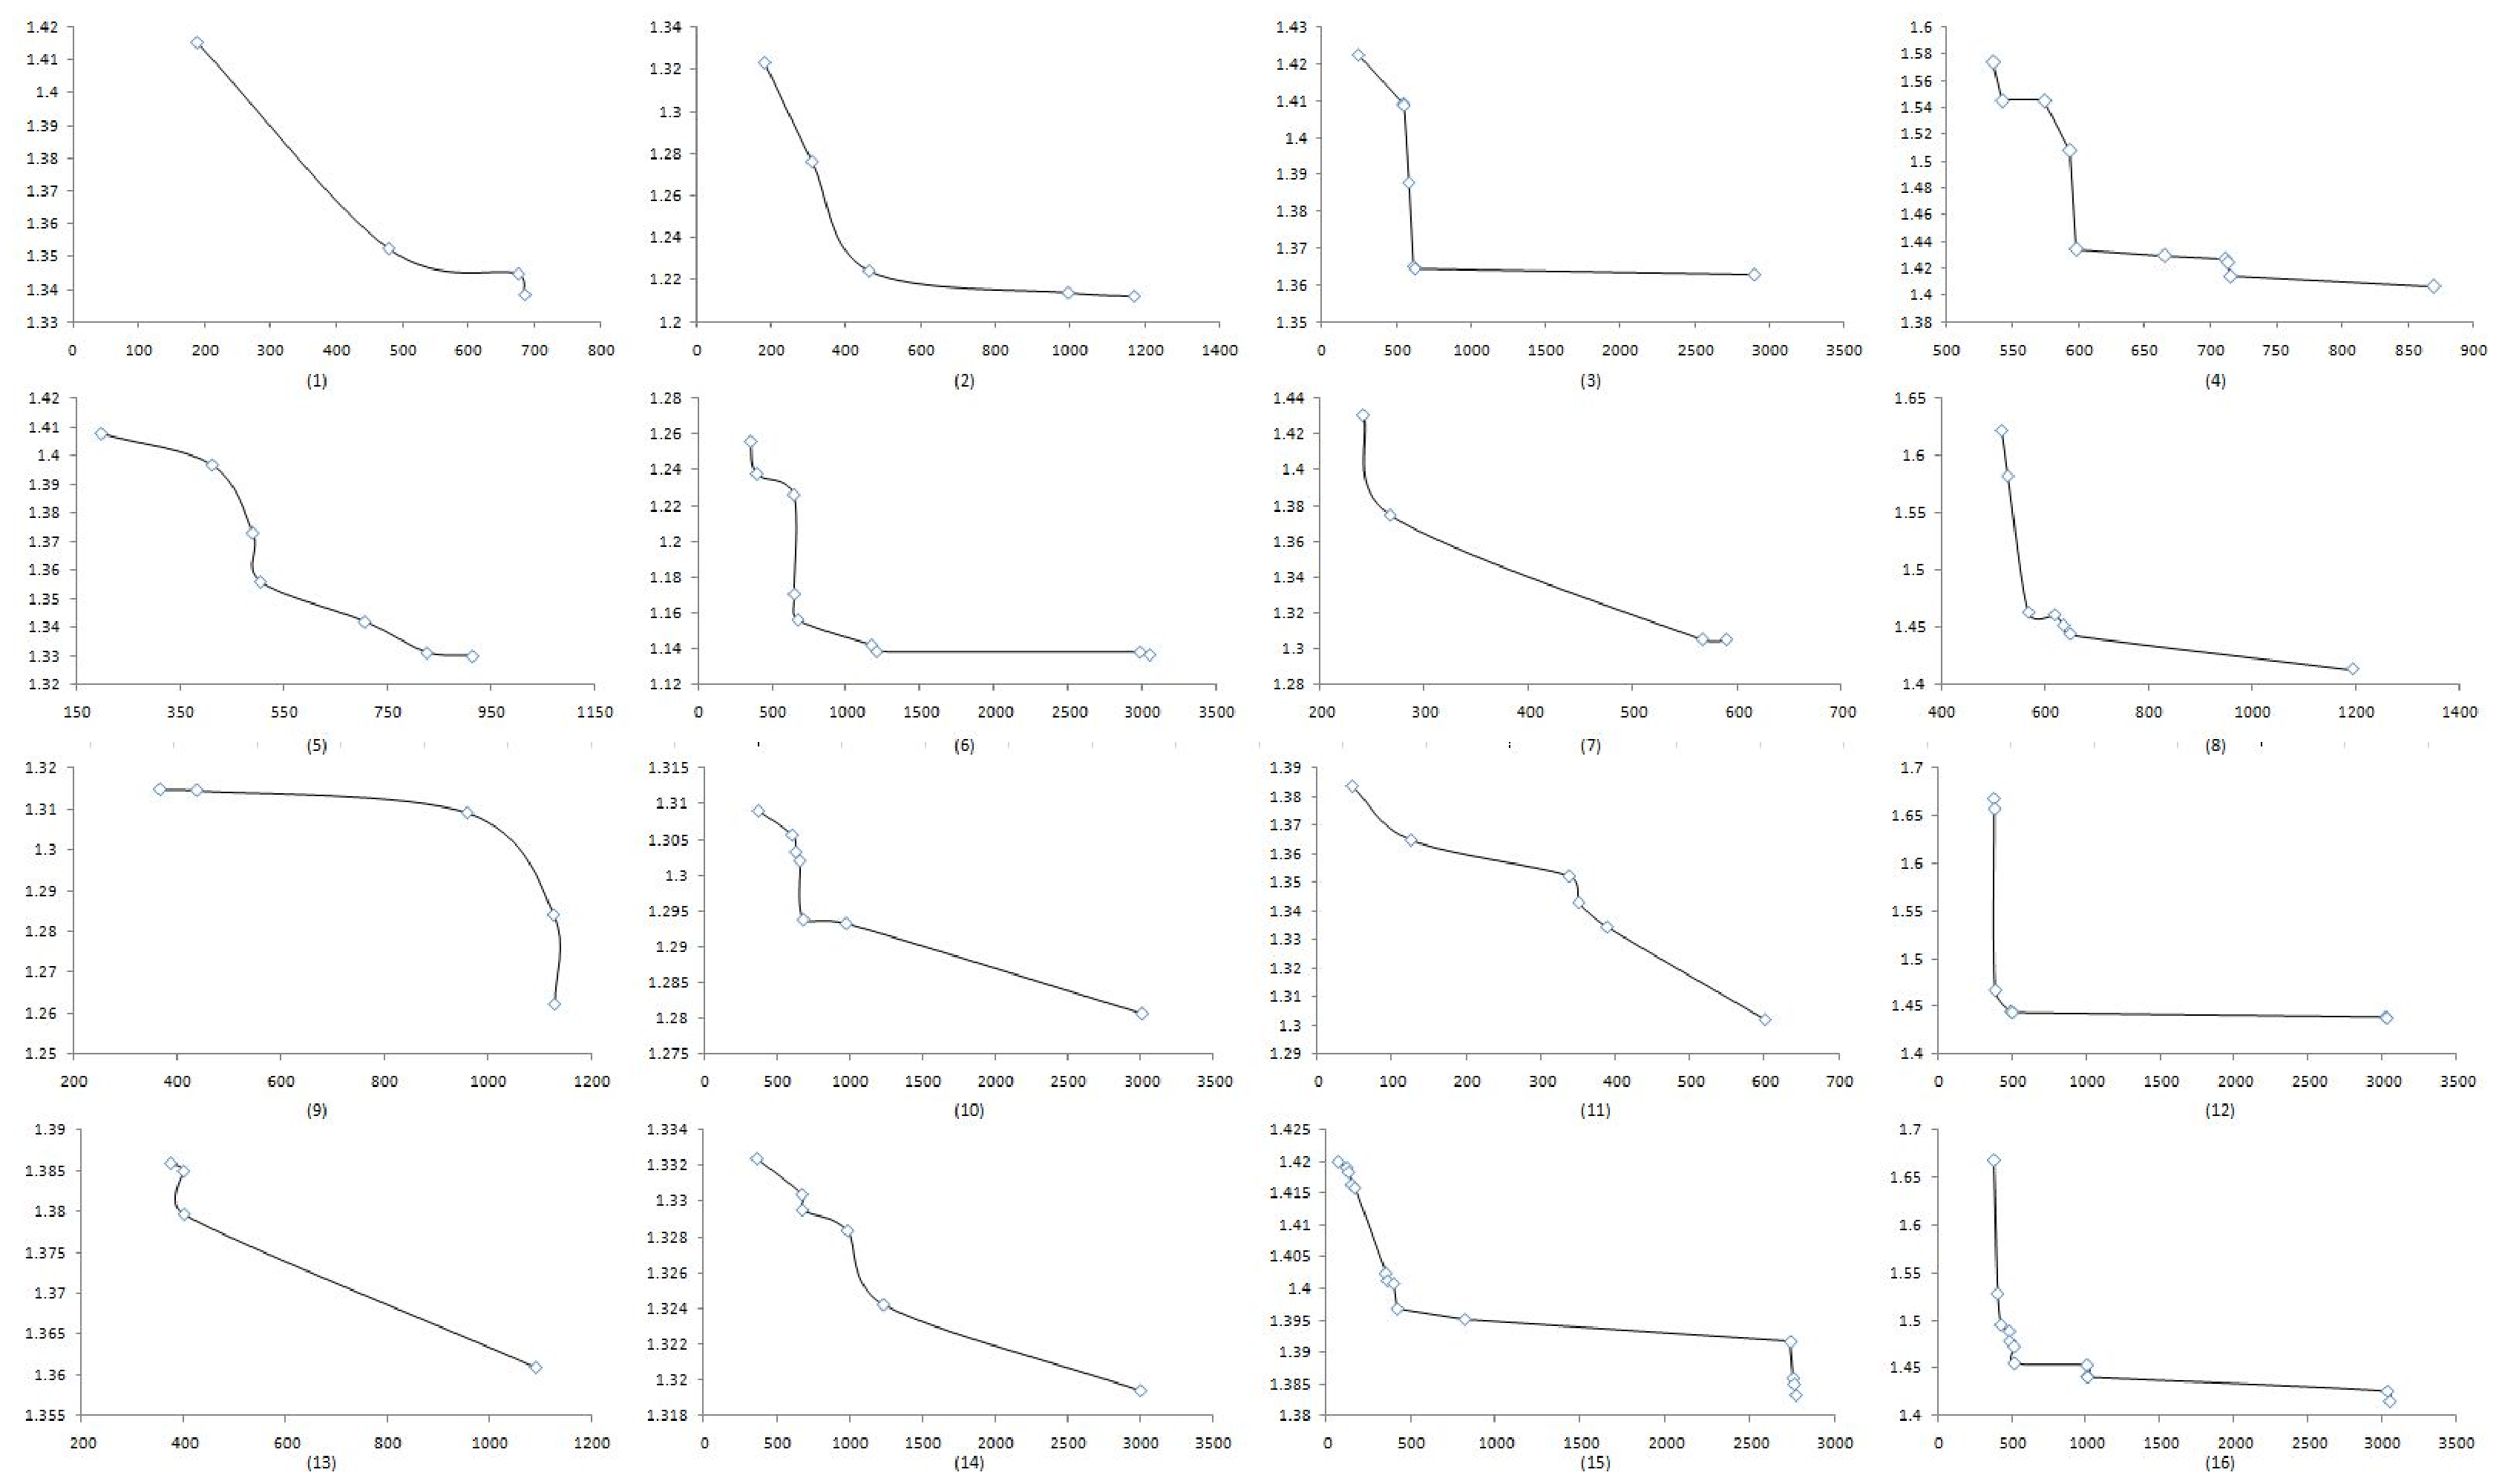
\includegraphics[width=1.\textwidth]{nemo_exp2.eps}
%\end{center}
%\caption{\label{fig:nemo_exp} Pareto fronts obtained from the 16 test cases of the neuroscience dataset.}
%\end{figure*}

It can be observed from the results in Table~\ref{tbl:nemo_perf} that more different factors involved in the acquisition of the two datasets for matching can negatively affect the matching performance. For example, in test case 1, the two datasets are drawn from the same subject group (SG1) and preprocessed using the same decomposition method (sICA); whereas in test case 4, the subject groups and decomposition methods are all different, resulting in greater variability and hence the performance is less satisfactory. However, it is worth noting that our method greatly outperforms traditional whole-attribute-based statistic characterization, as is shown in Figure~\ref{fig:perf_comp}. In this figure we also demonstrate the accuracy of the segmented statistics characterization with expert-labeled patterns, meaning that the data is partitioned and aligned in the most accurate way, which marks the best achievable attribute matching performance. But it is not feasible because, as mentioned in~Section~\ref{sec:intro}, manually recognizing patterns (partitioning data) and aligning them across datasets requires a priori knowledge of attributes in the datasets which is exactly what the problem of attribute matching tries to discover (the circular causality problem). On the other hand, our method does not require human involvement (except the specification of the number of clusters (patterns) present in the data in order to run the clustering analysis) in determining both the attribute matching and cluster matching and is able to achieve close-to-optimal results.

\begin{figure*}[tb]
\begin{center}
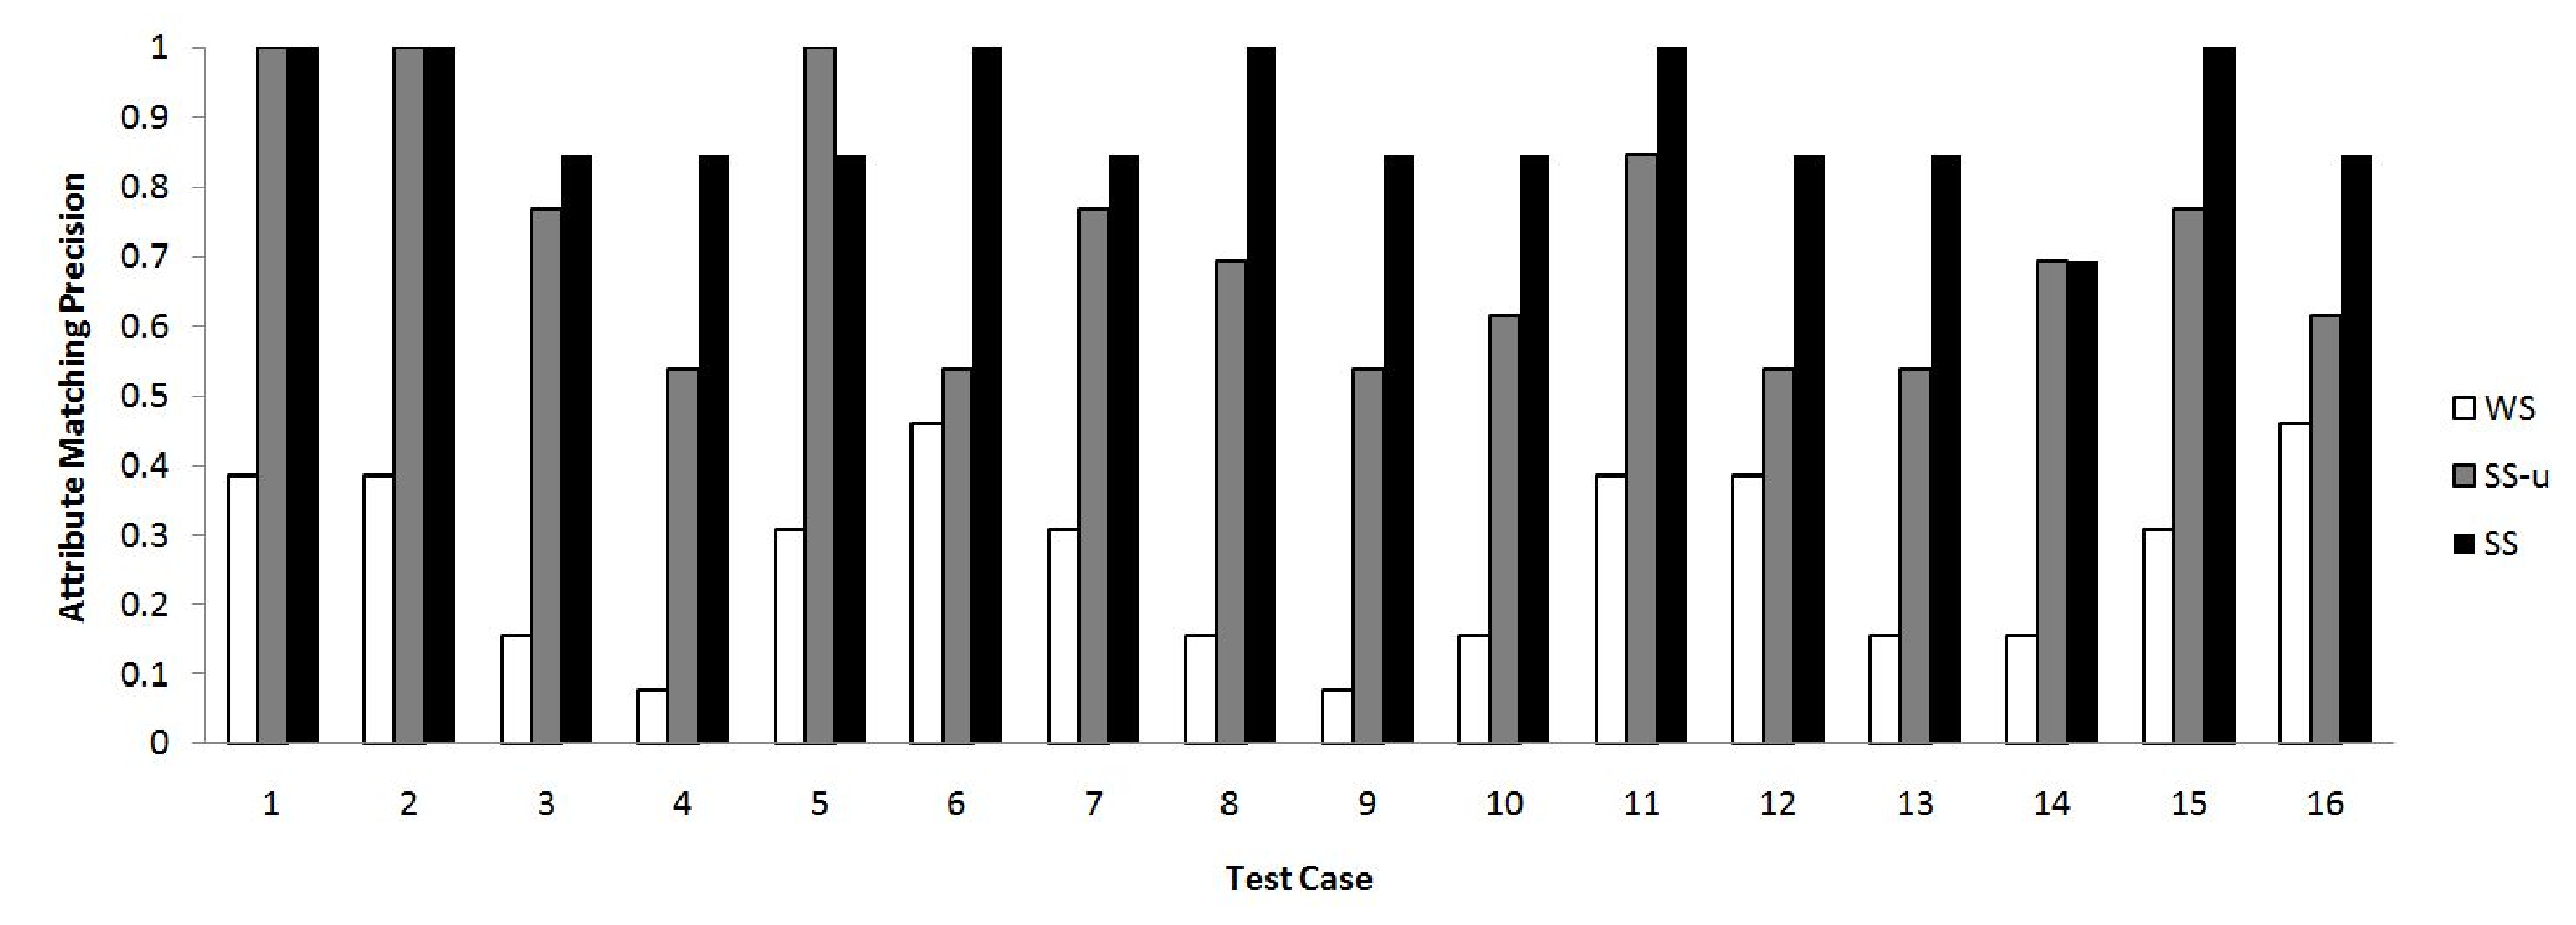
\includegraphics[width=1.\textwidth]{fig/perf_comp.eps}
\end{center}
\caption{\label{fig:perf_comp} A comparison of the attribute matching accuracy of three methods on the 16 test cases of the neuroscience dataset. The three methods being compared are matching based on whole-attribute statistics (WS), segmented attribute statistics without knowing a priori cluster matching (SS-u), and segmented attribute statistics with expert-aligned clusterings (SS).}
\end{figure*}


\begin{table*}[tbh]
\begin{center}
\begin{tabular}{l|l|l|l|l|l}
\hline
Test case & Source params & Target params & $~~~P_a~~~$ & $~~~P_c~~~$ & $|\Sigma|$\\
\hline
1		&	$\langle$	SG1, sICA, m1	$\rangle$	&	$\langle$	SG1, sICA, m2	$\rangle$	&		13/13	&	5/5	&	5	 \\
2		&	$\langle$	SG1, sICA, m1	$\rangle$	&	$\langle$	SG2, sICA, m2	$\rangle$	&		13/13	&	5/5	&	6	 \\
3		&	$\langle$	SG1, sICA, m1	$\rangle$	&	$\langle$	SG1, tPCA, m2	$\rangle$	&		10/13	&	5/5	&	6	 \\
4		&	$\langle$	SG1, sICA, m1	$\rangle$	&	$\langle$	SG2, tPCA, m2	$\rangle$	&		7/13	&	3/5	&	8	 \\
5		&	$\langle$	SG2, sICA, m1	$\rangle$	&	$\langle$	SG1, sICA, m2	$\rangle$	&		11/13	&	3/5	&	7	 \\
6		&	$\langle$	SG2, sICA, m1	$\rangle$	&	$\langle$	SG2, sICA, m2	$\rangle$	&		13/13	&	5/5	&	7	 \\
7		&	$\langle$	SG2, sICA, m1	$\rangle$	&	$\langle$	SG1, tPCA, m2	$\rangle$	&		10/13	&	5/5	&	6	 \\
8		&	$\langle$	SG2, sICA, m1	$\rangle$	&	$\langle$	SG2, tPCA, m2	$\rangle$	&		9/13	&	2/5	&	8	 \\
9		&	$\langle$	SG1, tPCA, m1	$\rangle$	&	$\langle$	SG1, sICA, m2	$\rangle$	&		7/13	&	5/5	&	4	 \\
10		&	$\langle$	SG1, tPCA, m1	$\rangle$	&	$\langle$	SG2, sICA, m2	$\rangle$	&		8/13	&	5/5	&	6	 \\
11		&	$\langle$	SG1, tPCA, m1	$\rangle$	&	$\langle$	SG1, tPCA, m2	$\rangle$	&		11/13	&	5/5	&	6	 \\
12		&	$\langle$	SG1, tPCA, m1	$\rangle$	&	$\langle$	SG2, tPCA, m2	$\rangle$	&		7/13	&	3/5	&	5	 \\
13		&	$\langle$	SG2, tPCA, m1	$\rangle$	&	$\langle$	SG1, sICA, m2	$\rangle$	&		7/13	&	3/5	&	5	 \\
14		&	$\langle$	SG2, tPCA, m1	$\rangle$	&	$\langle$	SG2, sICA, m2	$\rangle$	&		9/13	&	5/5	&	6	 \\
15		&	$\langle$	SG2, tPCA, m1	$\rangle$	&	$\langle$	SG1, tPCA, m2	$\rangle$	&		10/13	&	3/5	&	8	 \\
16		&	$\langle$	SG2, tPCA, m1	$\rangle$	&	$\langle$	SG2, tPCA, m2	$\rangle$	&		8/13	&	3/5	&	8	 \\
\hline
\end{tabular}
\end{center}
\caption{\label{tbl:nemo_perf} Matching performance of the proposed method with MOSA on the 16 test cases from the neuroscience dataset. The source and target parameter configuration of the data acquisition process of each test case are shown. $P_a$ and $P_c$ denote the accuracy of attribute matching and cluster matching respectively. $\Sigma$ is the number of points in the obtained Pareto-front. The quantities listed in the table are obtained by averaging over 5 runs of each test.}
\end{table*}

\subsection{Comparison with Multi-Objective Genetic Algorithm}
The concept of Genetic Algorithm (GA) was developed by Holland and his colleagues~\cite{Holland1992}. GA is first inspired by the evolutionary process in which weak and unfit species within their environment are faced with extinction and stronger ones have greater opportunities to pass their genes to next generation. Comparing to Simulated Annealing, Genetic Algorithm often offers a different perspective in the field of numerical optimization. Starts from a number of random generated population, cross over and evolve; GA has the ability to search in parallel around different and often fully scattered instances in the solution space, in contrast to the ``single thread" search in Simulated Annealing. In this paper, we also implemented the Multi-Objective Genetic Algorithm as the metaheuristics to solve the dual matching problem.

%For the crossover operation in our MOGA implementation, we go through all the attributes (clusters) in a random sequence, if the matching of one attribute in both parents is not used, we keep the matching from either one of its parents with 50\% probability; if the matching of one of the two parent is used, we keep the matching from another parent; or if the matching of both parents are used already, we random choose one matching from the rest used matching attribute.

To compare the performance between GA and SA, we first carry out an experiment on the same set of Neuroscience Data, as shown in Table~\ref{tbl:moga_neuro}. The iteration parameters of both algorithm are tuned so that the convergence time are about the same. The performance are then compared under such setting. We manually examine the Pareto front derived in each test case and find the solution that is closest to the gold standard and the accuracy of which is reported in Table~\ref{tbl:moga_neuro} (averaged over 5 independent runs).

\begin{table*}[tbh]
\begin{center}
\begin{tabular}{l|l|l|l}
\hline
Test Case	&	$P_a$ (\%)	&	$P_c$ (\%) &   $\Sigma$    \\
\hline
1	&	100	&	100	  &   9\\
2	&	98.2	&	96.6	&   10\\
3	&	53.4	&	98.0	 &  9\\
4	&	53.3	&	98.0	&   11\\
5	&	100	&	98.2	&    5\\
6	&	71.2	&	96.0	&   6\\
7	&	59.4	&	94.4	&   6\\
8	&	59.7	&	98.8	&   6\\
9	&	25.2	&	100.0	&6 \\
10	&	38.5	&	100.0	& 5\\
11	&	77.7	&	99.2	&  7\\
12	&	69.2	&	100.0	& 9\\
13	&	38.7	&	100.0	& 9\\
14	&	40.3	&	98.8	&  11\\
15	&	45.0	&	96.0	&  8\\
16	&	84.6	&	98.8	&  16\\
\hline
\end{tabular}
\end{center}
\caption{\label{tbl:moga_neuro} Matching performance of the proposed method with MOSA on the 16 test cases from the neuroscience dataset. The source and target parameter configuration of each test case is the same as in Table~\ref{tbl:nemo_perf}.}
\end{table*}

The number of population kept in each generation is an important parameter regarding the complexity and performance in MOGA. Intuitively, the more instances we keep, the broader the search space we can explore in each generation. Table~\ref{tbl:moga_neuro} shows the result with the number of population set to 4. We have also tested other settings and found out that the accuracy in most cases increase with the number of population but in rare cases the performance deteriorates. The overall performance of MOGA is comparable to that of MOSA but appears to be less robust. It is worth noting that the metaheuristics (MOSA and MOGA) we employed in the experiments are simple algorithms. More modern and sophisticated methods that explore various fitness assignment procedure, elitisim, or diversification approaches will be very likely to improve the performance.


\begin{table*}[tbh]
\begin{center}
\begin{tabular}{l||l|l||l|l}
\hline
 & \multicolumn{2}{c||}{mean} & \multicolumn{2}{c}{stdev}\\
\cline{2-5}
 & data1 & data2 & data1 & data2\\
\hline
\hline
fixed acidity & 6.86 & 6.85 & 0.84 & 0.86\\
volatile acidity & 0.28 & 0.28 & 0.1 & 0.1\\
citric acid & 0.34 & 0.33 & 0.12 & 0.12\\
residual sugar & 6.35 & 6.43 & 4.98 & 5.16\\
chlorides & 0.05 & 0.05 & 0.02 & 0.02\\
free sulfur diocide & 35.58 & 35.02 & 16.4 & 17.61\\
total sulfur dioxide & 138.98 & 137.68 & 41.86 & 43.18\\
density & 0.99 & 0.99 & 0.02 & 0\\
pH & 3.19 & 3.19 & 0.16 & 0.15\\
sulphates & 0.49 & 0.49 & 0.11 & 0.12\\
alcohol & 10.53 & 10.49 & 1.25 & 1.22\\
quality & 5.88 & 5.88 & 0.89 & 0.89\\
\hline
\end{tabular}
\end{center}
\caption{\label{tbl:wine_stat} Summary of the statistical characteristics of attributes in the Wine Quality dataset.}
\end{table*}

\subsubsection{Wine Quality Dataset}
In order to further validate our method, we implement our method also on a real-world wine quality dataset~\cite{CorCer09} which is available through the UCI machine learning repository\footnote[1]{\url{http://archive.ics.uci.edu/ml/datasets/Wine+Quality}}. This dataset has 12 attributes and 4898 records. We apply uniform sampling to split it into two equal-sized subsets. The attributes are anonymized and randomly reordered in each subset to generate artificial heterogeneity.

We then apply the proposed method with MOSA and MOGA as metaheuristics respectively. The test is focused on attribute matching because the gold standard is known while the gold standard of cluster matching is unknown. Table~\ref{tbl:wine_stat} summarizes the statistics for each attributes in the dataset. For both MOSA and MOGA derived Pareto optimal solutions, we manually select the one that is closest to the gold-standard matching (e.g., the solution with 10 out 12 attributes matched correctly). Each metaheuristics is invoked 5 times and the matching accuracy is averaged over these runs. The performance for attribute matching is shown in Table~\ref{tbl:wine_res}. The result demonstrate a markedly high accuracy for both MOSA and MOGA. It is worth noting that in most runs the Pareto fronts derived from MOSA and MOGA contain the gold standard matching (hence the high accuracy). It suggests a strategy to reduce the Pareto front in the matching problem by running MOSA or MOGA repeatedly after some times and only those ``stable" points that appear more than certain proportion of the times are considered to be presented to decision makers.

\begin{table*}[tbh]
\begin{center}
\begin{tabular}{c || c | c}
\hline
& accuracy (\%)	&	running time (ms)	\\
\hline
\hline
MOSA	&	95.5	&	517	\\
\hline
MOGA	&	92.3	&	3356\\
\hline
\end{tabular}
\end{center}
\caption{\label{tbl:wine_res} Performance of the proposed method with MOSA and MOGA as metaheuristics respectively on the Wine Quality dataset.}
\end{table*}


\section{Mining Semantically Associated Itemset}
\label{experiment}
Because we are interested in understanding the differences between the $s_{CT}$ and $s_{L+}$ similarity measures for generating semantically associated itemsets, we conducted a series of experiments to highlight their tradeoffs.  First, to illustrate the power of hypergraphs in finding associations via linking items, we synthesized a dataset for the \emph{fish oil} example.  Next, to illustrate the tradeoffs between the two methods, we evaluated both methods against a commonly used \emph{shopping cart} dataset.  Finally, encouraged by these results, we applied these methods to actual \emph{electronic health records} to highlight their scalability and applicability to the medical domain.

%In this section, we empirically evaluate the effectiveness and efficiency of the proposed methods. We use both low-dimensional and high-dimensional data sets in the experiments.

\subsection{Fish Oil}
\subsubsection{Dataset}
As mentioned in Section~\ref{sec:introduction}, \emph{fish oil} and \emph{Raynaud's syndrome} have been shown by Swanson~\cite{swanson87} to be linked together indirectly via various \emph{blood changes}.  He found these associations from examining biomedical texts.  As a proof of concept, we replicated this situation by synthesizing a table of 50 rows, which is about the same scale as in Swanson's experiment.  Each row represents a set of terms generated to represent biomedical text.   Each set of terms was specifically generated so that \emph{fish oil} and \emph{Raynaud's syndrome} never appear together. The column headers include \emph{fish oil, blood changes}, \emph{Raynaud's syndrome}.  Six other random variables acted as noise.  We then applied the $s_{CT}$, $s_{L+}$ to the dataset. Specifically, we set a threshold for first generating top-15 2-itemsets using either similarity measure. Based on the generated 2-itemsets we used clique search to generate $(k>2)$-itemsets.

%The goal of the synthetic data experiment is to show proof-of-concept of proposed method for discovering semantically associated itemsets by emulating the setting in Swanson's landmark paper [] published in 1987, in which he hypothesized that dietary fish oil could probably be used to treat Raynaud's syndrome by identifying, in some literature, associations between fish oil and blood change and, in some other literature, Raynaud's syndrome and blood change. The synthetic dataset is a relational table of 50 rows, just about the same scale as Swanson's experiment. Each row represents key terms (indicated by column headers) extracted from some imaginary biomedical publication (essentially a boolean bag-of-word representation in information extraction). The column headers include \texttt{fish\_oil, blood\_change}, \texttt{Raynaud\_syndrome} and six other random variables acted as noise. It is specifically made so that \texttt{fish\_oil} and \texttt{Raynaud\_syndrom} never occur together in the same row, corresponding to the setting of Swanson's experiment where no literature covers the association between those two.

\subsubsection{Results}
The hypergraph approach finds significant links between \emph{fish oil} and \emph{Raynaud's syndrome}, as demonstrated particularly well by the $s_{CT}$ method as shown in Table~\ref{tbl:syn}. Even the triplet was discovered by the clique search technique.  Most notably, because their co-occurrence is zero, the association would never be discovered by traditional frequent itemset techniques such as the Apriori algorithm~\cite{apriori}.

The $s_{L+}$ method also picks-up the association, but it was fairly weak:  the association is ranked 23rd among all 2-itemsets (column 3 in Table~\ref{tbl:syn} lists the ranking of the $s_{CT}$ results given by the $s_{L+}$).  However, as our next evaluations suggest, the $s_{L+}$ demonstrates other favorable qualities.
\begin{table}
\begin{center}
\begin{tabular}{r |@{ } r |@{ } r | l }
  \hline
  % after \\: \hline or \cline{col1-col2} \cline{col3-col4} ...
$\mathbf{s_{CT}}$  & $\mathbf{s_{L+}}$ rank    &\textbf{Freq}&   \textbf{Itemset}\\
  \hline\hline
0.83	&2&	25	&	$\langle$\emph{ blood\_change,	fish\_oil }$\rangle$\\
0.83	&1&	25	&	$\langle$\emph{ blood\_change,	Raynaud\_synd }$\rangle$\\
\textbf{0.79}	&\textbf{--}&	\textbf{0}	    &	$\langle$\emph{ \textbf{blood\_change,	fish\_oil,	Raynaud\_synd} }$\rangle$\\
0.76	&--&	10	&	$\langle$\emph{ blood\_change,	fish\_oil,	f }$\rangle$\\
0.76	&7&	16	&	$\langle$\emph{ blood\_change,	f }$\rangle$\\
0.76	&6&	16	&	$\langle$\emph{ blood\_change,	d }$\rangle$\\
0.76	&3&	16	&	$\langle$\emph{ blood\_change,	b }$\rangle$\\
%18.58	&	0	    &	$\langle$\emph{ blood\_change,	fish\_oil,	Raynaud\_synd,	a,	b,	c,	d,	e,	f }$\rangle$\\
0.75	&9&	15	&	$\langle$\emph{ blood\_change,	a }$\rangle$\\
0.75	&4&	15	&	$\langle$\emph{ blood\_change,	e }$\rangle$\\
0.73	&10&	14	&	$\langle$\emph{ blood\_change,	c }$\rangle$\\
\textbf{0.72}	&\textbf{23}&	\textbf{0}	    &	$\langle$\emph{ \textbf{fish\_oil,	Raynaud\_synd} }$\rangle$\\
0.70	&10&	10	&	$\langle$\emph{ fish\_oil,	f }$\rangle$\\
0.70	&--&	10	&	$\langle$\emph{ fish\_oil,	d }$\rangle$\\
0.70	&9&	9	&	$\langle$\emph{ fish\_oil,	b }$\rangle$\\
0.68	&20&	6   	&	$\langle$\emph{ Raynaud\_synd,	f }$\rangle$\\
  \hline
\end{tabular}
\end{center}
\caption{\label{tbl:syn} Top semantically associated itemsets generated by $s_{CT}$ from the Synthetic Fish Oil dataset.}
\end{table}


%We apply both $sim_{CT}$ and $sim_{L+}$ to generate semantically associated 2-itemsets and use the clique expansion to generate $(k>2)$-itemsets. Specifically, we set a threshold for first generating top-15 2-itemsets using either similarity measure, and use the derived 2-itemsets to prune the induced subgraph of the hypergraph model of the data. We then search for cliques in the resulting subgraph as $k$-itemsets. The final result obtained by $sim_CT$ is shown in table~\ref{tbl:syn} ordered according to the mean similarity score over the clique. We observe that the hypothetical itemsets $\langle$\emph{ \texttt{blood\_change,	fish\_oil,	 Raynaud\_synd} }$\rangle$ and $\langle$\emph{ \texttt{fish\_oil,	Raynaud\_synd} }$\rangle$ all appear in this top list according to $sim_{CT}$. The frequency of their co-occurrence is zero, therefore never will they be considered as traditional frequent itemsets. The result obtained by $sim_{L+}$ is not shown because the $\langle$\emph{ \texttt{fish\_oil,	Raynaud\_synd} }$\rangle$ is ranked 23th among all 2-itemsets thus following below the threshold. Despite that $sim_{L+}$ fail to rank the desired itemsets high enough, it still assigns a non-zero score to it. We will soon see the effect of $sim_{L+}$ on real datasets demonstrating its capability to capture some unique pattern. The synthetic data experiment shows that the proposed method is indeed capable of discovering semantically associated itemsets by utilizing indirect connections through linking items.


\subsection{Shopping Cart}
\subsubsection{Dataset}
To better understand how the $s_{CT}$ method compares against the $s_{L+}$ method, we tested them on a business shopping cart dataset.  This dataset contains purchase information on 100 grocery items (represented by boolean column headers) for 2,127 shopping orders (corresponding to tuples). We applied $s_{L+}$ and $s_{CT}$ and set a threshold to include top-100 2-itemsets, based on which we subsequently used clique search to generate $(k>2)$ itemsets. The top-10 2-itemset results and ($k>2$)-itemsets corresponding to maximum cliques generated by $s_{CT}$ and $s_{+}$ are reported in Table~\ref{tbl:foodmart_ct} and \ref{tbl:foodmart_pl} respectively.

% this data set is interesting because... why? it is used by many in classrooms? it is just the right size?  it is easily understandable?  what?  give a motivation of somekind for choosing it xxx



\subsubsection{Results}
Unlike the experiment on the fish oil dataset, We do not have specific hypothesis to validate in this test. After examining the results from both measures, we can only conclude they make intuitive sense. However, we observe that the difference between the $s_{CT}$ and $s_{L+}$ becomes more significant in this experiment. The $s_{CT}$ tends to include itemsets with high support and the effect of indirect links is less pronounced. On the other hand, $s_{L+}$ promotes items with support values towards the lower end. We also observe one drawback of the $s_{CT}$ that the result is centered around items with large frequencies (i.e., many direct links to other nodes) and hence in a sense limiting the information (most itemsets are about \emph{cheese}, \emph{soup} and \emph{cookie}). By contrast, the $s_{L+}$ produces more diversified itemsets.

Finally we tested our methods on the dataset of electronic health records of real patients. This dataset is different from the above two datasets not only in scale but also in practical importance as described in the following.
% state in very clear sentence what the conclusion is, what is the take-home message you want them to see? xxx

% why is this interesting? what should we have learned? xxx

%finally, lead-in to final experiment... we finally did this last experiment because:  1) its huge, 2) its important to people to solve xxx

\begin{table}
\begin{center}
\begin{tabular}{l|l | l | l }
  \hline
  % after \\: \hline or \cline{col1-col2} \cline{col3-col4} ...
&$\mathbf{s_{CT}}$       &\textbf{Freq}&   \textbf{Itemset}\\
  \hline\hline
\multirow{10}{*}{2-itemsets}& 0.74	&	39	&$\langle$\emph{	Cheese,	Soup	}$\rangle$\\
&0.73	&	32	&$\langle$\emph{	Cheese,	Dried Fruit	}$\rangle$\\
&0.72	&	36	&$\langle$\emph{	Dried, Fruit	Soup	}$\rangle$\\
&0.72	&	38	&$\langle$\emph{	Cookies,	Soup	}$\rangle$\\
&0.71	&	24	&$\langle$\emph{	Cheese,	Cookies	}$\rangle$\\
&0.70	&	30	&$\langle$\emph{	Cookies,	Dried Fruit	}$\rangle$\\
&0.68	&	31	&$\langle$\emph{	Cheese,	Preserves	}$\rangle$\\
&0.67   &	24	&$\langle$\emph{	Cheese,	Wine	}$\rangle$\\
&0.67	&	21	&$\langle$\emph{	Preserves,	Soup	}$\rangle$\\
&0.67	&	28	&$\langle$\emph{	Soup,	Wine	}$\rangle$\\
%102.7534	&	21	&$\langle$\emph{	Cheese,	Nuts	}$\rangle$\\
\hline
\parbox{1cm}{$(k$$>$2$)$-itemsets}&0.64 &	0	&\parbox{6cm}{$\langle$\emph{ Canned Vegetables, Cheese, Cookies, Dried Fruit, Frozen Vegetables, Nuts, Preserves, Soup, Wine }$\rangle$}\\
  \hline
\end{tabular}
\end{center}
\caption{\label{tbl:foodmart_ct} Top semantically associated itemsets generated by $s_{CT}$ from the shopping cart dataset.}
\end{table}

\begin{table}
\begin{center}
\begin{tabular}{l|l| l | l }
  \hline
  % after \\: \hline or \cline{col1-col2} \cline{col3-col4} ...
&$\mathbf{s_{L+}}$       &\textbf{Freq}&   \textbf{Itemset}\\
  \hline\hline
\multirow{10}{*}{2-itemsets}& 10.17	&	3	&$\langle$\emph{	Sardines,	Conditioner	}$\rangle$\\
&8.17	&	6	&$\langle$\emph{	Toothbrushes,	Nasal Sprays	}$\rangle$\\
&6.70	&	6	&$\langle$\emph{	Yogurt,	Anchovies	}$\rangle$\\
&6.25	&	5	&$\langle$\emph{	Sports Magazines,	Cottage Cheese	}$\rangle$\\
&5.82	&	5	&$\langle$\emph{	Tofu,	Sour Cream	}$\rangle$\\
&5.79	&	3	&$\langle$\emph{	Toothbrushes,	Acetominifen	}$\rangle$\\
&4.77	&	4	&$\langle$\emph{	Sauces,	Nasal Sprays	}$\rangle$\\
&4.46	&	3	&$\langle$\emph{	Sports Magazines,	Gum	}$\rangle$\\
&4.43	&	4	&$\langle$\emph{	Sunglasses,	Paper Dishes	}$\rangle$\\
&4.05	&	5	&$\langle$\emph{	Tofu,	Canned Fruit	}$\rangle$\\
  \hline
\multirow{3}{*}{\parbox{1cm}{$(k$$>$2$)$-itemsets}}&4.51	&	2	&$\langle$\emph{	Canned Fruit,	Sour Cream,	Tofu	 }$\rangle$\\
&2.01	&	1	&$\langle$\emph{	Batteries,	Cereal,	Cooking Oil	}$\rangle$\\
&1.75	&	5	&$\langle$\emph{	Canned Vegetables,	Nuts,	Waffles	}$\rangle$\\
\hline
\end{tabular}
\end{center}
\caption{\label{tbl:foodmart_pl} Top semantically associated itemsets generated by $s_{L+}$ from the shopping cart dataset.}
\end{table}

\subsection{Electronic Health Records}
\subsubsection{Dataset}
In our final evaluation, we analyzed the electronic health records of real patients. Applying methods like the ones we have described to this kind of data is particularly relevant because of recent legislation aimed at increasing the meaningful use of electronic health records. Discovering meaningful semantically associated itemsets among the set of drugs and diseases identified in the patient's clinical note is a critical step toward identifying combinations of drug classes and co-morbidities, or risk-factors and co-morbidities that are common in patients with a certain outcome (for example, those suffering from myocardial infarction), toward building predictive risk models, as well as toward providing probable hypotheses about the possible causes of that outcome.  %The main challenge is that roughly 80\% of the clinical electronic medical data is found in free-text narrative (e.g., doctor's notes).

We obtained the set of drugs and diseases for each patient's clinical note by using a new tool, the \emph{Annotator Workflow}, developed at the National Center for Biomedical Ontology (NCBO).  The patient notes are from Stanford Hospital's Clinical Data Warehouse (STRIDE).  These records archive over 17-years worth of patient data comprising of 1.6 million patients, 15 million encounters, 25 million coded ICD9 diagnoses, and a combination of pathology, radiology, and transcription reports totaling over 9 million clinical notes (i.e., unstructured text).

%In addition to having obvious data-mining applications, the workflow has been used by biomedical researchers to build semantic-search applications, such as the NCBO Resource Index~\cite{jonquet11}, which won the Semantic Web Challenge\footnote{\url{http://challenge.semanticweb.org/}} in 2010. The annotation process utilizes the vast NCBO BioPortal ontology library~\cite{bioportal} to extract information by using a lexicon of over one million terms generated from the relevant ontologies, such as SNOMED-CT, RxNORM, and MedDRA. Furthermore, it also incorporates negation detection --- the ability to discern whether a term is negated with the context of the narrative (e.g., lack of valvular dysfunction). Finally, it uses mappings between terms across ontologies~\cite{ghazvinian09}, which forms a rich knowledge graph %(Figure~\ref{fig:collapse})
%or mega-thesaurus, to normalize the lexicon by reducing the feature set from over one million to merely 11,107 unique drugs and 3,594 unique diseases.

From this set of 1.6 million patients, we extracted a cohort of patients that suffered from kidney failure.  Out of those records, we applied our algorithms to all previous records in the patient's timeline, looking at just the set of drugs.  Therefore, at a very simplistic level, the experiment result shows that semantically associated itemsets in this context could possibly represent sets of drugs that could lead toward kidney failure when used in combination.

%\begin{figure*}[tbh]
%\centering
%\includegraphics[width=.8\textwidth]{fig/collapse2.eps}
%%\vskip -0.75em
%\caption{The \textbf{knowledge graph}:  The knowledge graph formed by the relationships in drug and disease ontologies and the mappings between terms belonging to different ontologies. The figure shows a subsection of a disease hierarchy (red) and a drug hierarchy (blue) from the mega-thesaurus at BioPortal. Each node represents a class. The numbers (M=538,638 and N=535,410) show the total number of different terms from the mega-thesarus. The numbers (m=2,966 and n=11,107) in the inner circles show the count of classes that remain after collapsing along various relationships (e.g., synonymy, ingredient\_of, has\_tradename, is\_a) across all ontologies. The normalization resulting from collapsing the terms in clinical notes to such a knowledge graph results in a significant reduction in computation complexity.}
%\label{fig:collapse}
%%\vskip -0.75em
%\end{figure*}

%As a result of applying this tool to the patient records from STRIDE, we created a bit-map of roughly 9 million rows and 15 thousand columns.  Each row represents a patient note.  Each column represents either a drug or a disease (or a class of drug or class of disease).  The bit (1 or 0) represents either the presence or absence of a non-negated mention of the drug or disease in the note.  Each note (i.e., row) is linked to a patient identifier, a relative timestamp, and the patient's age\footnote{All ages approaching 90 are appropriately masked for privacy as required by law.} at the time so that the patient's timeline-view is preserved.  Other demographic data such as ethnicity and race were not used for this study.

\subsubsection{Results}
The cohort dataset described above contains 467791 rows (corresponding to patients' clinical notes) and 10167 columns (corresponding to annotated terms appeared in the notes). With the help of the techniques described in Section~\ref{sec:eff_comp}, we are able to compute $L^+$ in a tractable amount of time (Equation~\ref{eq:combinatoryHyperL} and \ref{eq:pL} are calculated within 4 hours on a Quad-Core AMD Opteron(tm) Processor with 8 gigabyte memory), based on which we can efficiently derive the $s_{L+}$ itemsets. However, the calculation of $s_{CT}$ on this scale is intractable because an exact computation of all pair-wise $s_{CT}$ requires to fill in a $|V|\times|V|$ similarity table. In order to ameliorate the computational cost, we exploit domain knowledge to identify 582 terms of particular interest and then apply both $s_{CT}$ and $s_{L+}$ on the reduced dataset. The results are shown in Table~\ref{tbl:ncbo_ct} and \ref{tbl:ncbo_lp} respectively, where we list top-10 2-itemsets and all ($k>$2)-itemsets corresponding to the maximum clique.

\begin{table}
\begin{center}
\begin{tabular}{l|c|c }
\hline
&\multicolumn{2}{c}{Support} \\
\hline
              & Shopping cart  &  Electronic health\\
\hline
$\mathbf{s_{CT}}$    & 0.58  & 0.82 \\
\hline
$\mathbf{s_{L+}}$    & 0.32  & 0.06 \\
\hline
\end{tabular}
\end{center}
\caption{\label{tbl:kendall} The Kendall-$\tau$ score between rankings of itemsets generated by $s_{CT}$, $s_{L+}$ and support in the two experiments.}
\end{table}

\begin{table}
\begin{center}
\begin{tabular}{l|l |l |l }
  \hline
  % after \\: \hline or \cline{col1-col2} \cline{col3-col4} ...
&$\mathbf{s_{CT}}$      &\textbf{Freq}&   \textbf{Itemset}\\
  \hline\hline
\multirow{10}{*}{2-itemsets}& 0.80	&	39204		&$\langle$\emph{	Calcium Chloride,	Amiloride	}$\rangle$\\
&0.77	&	29325		&$\langle$\emph{	Calcium Chloride,	Aspirin	}$\rangle$\\
&0.76	&	28644		&$\langle$\emph{	Calcium Chloride,	Probenecid	}$\rangle$\\
&0.73	&	24805		&$\langle$\emph{	Calcium Chloride,	Furosemide	}$\rangle$\\
&0.72	&	34271		&$\langle$\emph{	Calcium Chloride,	Calcium	}$\rangle$\\
&0.71	&	21481		&$\langle$\emph{	Calcium Chloride,	Disulfiram	}$\rangle$\\
&0.70	&	16814		&$\langle$\emph{	Calcium Chloride,	Amphetamine	}$\rangle$\\
&0.66	&	19850		&$\langle$\emph{	Calcium Chloride,	Prednisone	}$\rangle$\\
&0.65	&	12231		&$\langle$\emph{	Aspirin,	Amiloride	}$\rangle$\\
&0.65	&	12106		&$\langle$\emph{	Probenecid,	Amiloride	}$\rangle$\\
  \hline
\parbox{1cm}{$(k$$>$2$)$-itemsets}&0.56	&	0	&	\parbox{6cm}{$\langle$\emph{	Calcium Chloride, Disul-firam, Amphetamine, Aceta-minophen, Calcium, Aspirin, Probenecid, Amiloride, Prednisone, Furosemide	}$\rangle$}\\
\hline
\end{tabular}
\end{center}
\caption{\label{tbl:ncbo_ct} Top semantically associated itemsets generated by $s_{CT}$ from the kidney failure cohort of the electronic health dataset.}
\end{table}


\begin{table}
\begin{center}
\begin{tabular}{l |l | l | l }
  \hline
  % after \\: \hline or \cline{col1-col2} \cline{col3-col4} ...
&$\mathbf{s_{L+}}$      &\textbf{Freq}&   \textbf{Itemset}\\
  \hline\hline
\multirow{10}{*}{2-itemsets}&	0.820	&	354	&$\langle$\emph{	sevoflurane,	remifentanil	}$\rangle$\\
&	0.691	&	978	&$\langle$\emph{	frovatriptan,	almotriptan	}$\rangle$\\
&	0.633	&	693	&$\langle$\emph{	Etomidate,	Rocuronium	}$\rangle$\\
&	0.496	&	234	&$\langle$\emph{	Atazanavir,	Pyrimethamine	}$\rangle$\\
&	0.420	&	3004	&$\langle$\emph{	ciclesonide,	Fluorometholone	}$\rangle$\\
&	0.377	&	231	&$\langle$\emph{	naratriptan,	Mefenamic Acid	}$\rangle$\\
&	0.373	&	1792	&$\langle$\emph{	ciclesonide,	Vincristine	}$\rangle$\\
&	0.332	&	92	&$\langle$\emph{	Rocuronium,	sevoflurane	}$\rangle$\\
&	0.325	&	1368	&$\langle$\emph{	tazarotene,	halobetasol propionate	}$\rangle$\\
&	0.322	&	506	&$\langle$\emph{	Buprenorphine,	alosetron	}$\rangle$\\
  \hline
\parbox{1cm}{$(k$$>$2$)$-itemsets}&	0.131	&	701	&\parbox{6cm}{$\langle$\emph{	Ketorolac, Flurbiprofen, Ketorolac, Etodolac, Sulindac, Piroxicam, Ketoprofen	}$\rangle$}\\
\hline
\end{tabular}
\end{center}
\caption{\label{tbl:ncbo_lp} Top semantically associated itemsets generated by $s_{L+}$ from the kidney failure cohort of the electronic health dataset.}
\end{table}
It is clear that, continuing the trend shown in the FoodMart analysis, the $s_{CT}$ result becomes increasingly concordant with the support-based method. For illustrating this point of view, we calculate the Kendall-$\tau$ score between the ranking of itemsets generated by $s_{CT}$, $s_{L+}$, and support as shown in Table~\ref{tbl:kendall}. We observe from the table that as the $s_{CT}$ converges to support, the $s_{L+}$ becomes even more distinct from it. The result is that the itemsets discovered by $s_{CT}$ contain mostly general terms that are repeatedly found in the patients' notes. Although the association is reasonable but hardly interesting. On the contrary, the $s_{L+}$ result is not affected by the dimension of data as well as the presence of items with massive support. It identifies itemsets of relatively low support but more closely bonded by indirect links.

To demonstrate the scalability of the method based on the $s_{L+}$, we also conducted the same analysis on the data of the whole cohort after 2010. The data consisted 1 million rows and 10 thousand columns. We were able to produce the $s_{L+}$ based 2-itemsets in 6 hours. The top results are shown in Table~\ref{tbl:ncbo_lp_whole}.

The discovered $s_{L+}$ itemsets provide much valuable insights on the possible interrelationship between drugs. Some of them has been studied in the literature. For example, \emph{sevoflurane/remifentanil} can be used for anaesthesia; \emph{frovatriptan} and \emph{almotriptan} are both oral treatment of migraine headache; \emph{Etomidate} and \emph{Rocuronium} can be used for rapid sequence intubation; etc. This area of research is still very new and there are no good gold standards to compare our results against.  However, for single-item drugs that lead to kidney failure, SIDER\footnote{\url{http://sideeffects.embl.de/se/C0035078/all}} database lists drugs and their side-effects.  Most notably, multi-itemsets are difficult to identify, but our methods have found not only \emph{Ketoprofen} but it has also group other drugs like it (see the ($k>2$)-itemset shown in Table~\ref{tbl:ncbo_lp}, all of the items are anti-inflammatories). Our results are a matter of on-going evaluation with medical experts.


\begin{table}
\begin{center}
\begin{tabular}{l | l }
  \hline
  % after \\: \hline or \cline{col1-col2} \cline{col3-col4} ...
$\mathbf{s_{L+}}$      &   \textbf{Itemset}\\
  \hline\hline
0.0301	&$\langle$\emph{	White faced hornet venom, Yellow hornet venom		}$\rangle$\\
0.0195	&$\langle$\emph{	Trichloroacetic Acid, Trichloroacetate		}$\rangle$\\
0.0108	&$\langle$\emph{	Cloxacillin Sodium, benzathine cloxacillin		}$\rangle$\\
0.0101	&$\langle$\emph{	Methacycline, Methacycline hydrochloride		}$\rangle$\\
0.01	&$\langle$\emph{	Entamoebiasis, Hepatic, Liver Abscess, Amebic		}$\rangle$\\
0.0086	&$\langle$\emph{	butenafine, Butenafine hydrochloride		}$\rangle$\\
0.0085	&$\langle$\emph{	Acetone, Cantharidin		}$\rangle$\\
0.0085	&$\langle$\emph{	ethyl cellulose, Cantharidin		}$\rangle$\\
0.0085	&$\langle$\emph{	ethyl cellulose, Acetone		}$\rangle$\\
0.0085	&$\langle$\emph{	Poloxamer 407, Eucalyptol		}$\rangle$\\
  \hline
\end{tabular}
\end{center}
\caption{\label{tbl:ncbo_lp_whole} Top semantically associated itemsets generated by $s_{L+}$ from the whole electronic health dataset after 2010. The dataset contains 1 million rows and 10k columns.}
\end{table}

\section{Mining Semantic Association with Ontologies}
In this section, we evaluate the combined RDF bipartite graph for discovering semantic associations. We conducted a series of experiments to highlight the effect of the incorporation of ontologies in the mining framework, and to explore the impact of different ratios of weights assigned to various kinds of relationships in the graphs. First, to illustrate the power of combined RDF bipartite graph in finding semantic associations while taking into account seamlessly the ontological information, we evaluated our methods against a commonly used \emph{shopping cart} dataset together with a manually created ontology describing the subsumption hierarchy for grocery items.  Then, encouraged by the result, we applied our method to actual \emph{electronic health records} to highlight its scalability and applicability to the medical domain. The sizes of the datasets are specified in Table~\ref{tbl:exp_overview}.

\begin{table}[tbh]\scriptsize
\begin{center}
\begin{tabular}{c|c|c|c}
\hline
    & \# data stmts & \# isa stmts & \# other stmts* \\
    \hline
  Shopping cart     &  8,481       & 127       &    0\\
  Electronic health &  10,000,257  & 1,048,604 &    43780\\
  \hline
\end{tabular}
\end{center}
\caption{\label{tbl:exp_overview} Dataset overview (``stmts" stands for RDF statements). *In the electronic healths test, we explore the ``may\_treat" relationship between drugs and diseases defined in the National Drug File.}
\end{table}


\subsection{Shopping Cart}
\subsubsection{Dataset}
The shopping cart dataset contains purchase information on 100 grocery items (represented by boolean column headers) for 2,127 shopping orders (corresponding to tuples) from a Foodmart. We first construct an RDF bipartite graph from the dataset by transforming the table to 8481 RDF statements. Then we manually create an ontology to organize the grocery items into a subsumption hierarchy. In this process, we introduce 28 internal nodes (the 100 grocery items appeared in the data are mostly at the leaf level) and thus derive a total of 127 RDF statements. As the size of this dataset is fairly small, the calculation of similarity ranking for a given term is fast. In the following we highlight the effect of incorporation of ontology by comparing results obtained with and without ontologies.


\subsubsection{Results}
In Table~\ref{tbl:foodmart_comp}, results of items ranked by the strength of semantic association given a query term ``Toothbrush" under various combinations of parameters are demonstrated side-by-side for comparison. First, we observe that without using ontology, performing random walk with restart on the data graph (Table~\ref{tbl:foodmart_comp}.A) starting from ``toothbrush" yields similar results to those reported in our previous work~\cite{LiuEtal11} based on random walk commute time similarity. Items ranked high in this setting where only the data graph is considered are typically either hub nodes (with many edges linking to other items) or frequently co-occur with the query item (many edges connecting them). Second, applying the same similarity ranking method solely on the ontology graph (Table~\ref{tbl:foodmart_comp}.B) gives a list of association based on the graph-configuration of the ontological structure (in this case, the rdfs:subClassOf lattice). The items that are considered most similar to the query term ``Toothbrush" is its immediate parent class ``PersonalHygiene," followed by some most derived classes at the same level of ``PersonalHygiene" and then siblings of ``Toothbrush" itself. Next, Table~\ref{tbl:foodmart_comp}.C--E demonstrate the results of mining on the combined graph with different ratios of weights assigned to ontology edges and data edges respectively. It is obvious that these results can be seen as a mix of the data-only and ontology-only results with various emphasis on the data or ontology. We can observe that when $w_o/w_d=20$ where $w_o$ is weight of ontology edge (i.e., rdfs:subClassOf) and $w_d$ is the weight of data edge, the ontology and data appear to have equal significance in determining the ranking. In a rough sense, it conforms to the ratio of the size of ontology graph and data graph as well (see Table~\ref{tbl:exp_overview}). In reality, the appropriate ratio for the edge weights is not only dependent on the size of graphs but also the graph configuration (depth, average degree, etc). Moreover, specifying the ratio of prior knowledge in ontologies and inductive evidences in data that one wants to employ for discovering new patterns is a highly empirical process. Multiple pilot trials may need to be carried out for the optimal ratio before it is applied to the real application.

\begin{table*}[tbh]\scriptsize
\begin{center}
\begin{tabular}{ c c || c c || c c }
\hline
\multicolumn{2}{c||}{w/ data only}&\multicolumn{2}{c||}{w/ onto only}&\multicolumn{2}{c||}{$w_o=1$, $w_d=1$}\\
\hline
item	&	p(\%)	&	item	&	p(\%)	&	item	&	p(\%)	\\
\hline																			
Soup	&	0.42	&	PersonalHygiene	&	12.55	&	PersonalHygiene	&	0.74	\\
Cookies	&	0.41	&	Snack	&	0.86	&	Soup	&	0.41	\\
NasalSprays	&	0.38	&	Health	&	0.64	&	Cookies	&	0.4	\\
Popcorn	&	0.32	&	Sponges	&	0.57	&	NasalSprays	&	0.37	\\
PaperWipes	&	0.29	&	Soap	&	0.57	&	Popcorn	&	0.31	\\
FrozenVegetables	&	0.29	&	Shampoo	&	0.57	&	FrozenVegetables	&	0.29	 \\
PersonalHygiene	&	0.26	&	NasalSprays	&	0.57	&	PaperWipes	&	0.28	 \\
DriedFruit	&	0.25	&	Mouthwash	&	0.57	&	DriedFruit	&	0.25	 \\
Milk	&	0.25	&	Conditioner	&	0.57	&	Milk	&	0.25	\\
Mouthwash	&	0.24	&	MealCourse	&	0.54	&	Mouthwash	&	0.23	\\
\hline
\multicolumn{6}{c}{~}\\
\multicolumn{2}{c}{(A)}  &   \multicolumn{2}{c}{(B)}  &   \multicolumn{2}{c}{(C)}  \\
\multicolumn{6}{c}{~}\\
\end{tabular}

\begin{tabular}{ c c || c c }
\hline
\multicolumn{2}{c||}{$w_o=10$, $w_d=1$}&\multicolumn{2}{c}{$o_w=20$, $o_d=1$}\\
\hline
item	&	p(\%)	&	item	&	p(\%)	\\
\hline																			
PersonalHygiene	&	3.97	&	 PersonalHygiene	&	6.27	\\
NasalSprays	&	0.41	&	NasalSprays	&	0.5	\\
Soup	&	0.34	&	Mouthwash	&	0.41	\\
Cookies	&	0.34	&	Shampoo	&	0.31	\\
Mouthwash	&	0.3	&	Soup	&	0.29	\\
Popcorn	&	0.25	&	Cookies	&	0.29	 \\
FrozenVegetables	&	0.24	&	Sponges	&	0.28	 \\
PaperWipes	&	0.23	&	Health	&	0.27	 \\
DriedFruit	&	0.22	&	Conditioner	&	0.27	\\
Milk	&	0.21	&	Soap	&	0.25	\\
\hline
\multicolumn{4}{c}{~}\\
\multicolumn{2}{c}{(D)}  &  \multicolumn{2}{c}{(E)}  \\
\end{tabular}
\end{center}
\caption{\label{tbl:foodmart_comp} Foodmart items ranked by the strength of semantic association (i.e., $p(\%)$, the steady-state probability).}
\end{table*}

Note that without filtering the ranked semantic associations on the combined graph, the list will include items that never appear in the transactional data. It is because typically the semantic annotation process links table attributes to their most specific matching concept in the ontology which are close to the leaf level. The incorporation of ontology is to aid the mining process, therefore including in the result those internal items (e.g., ``PersonalHygiene") that never appear in the data is counterintuitive. To overcome this, we can simply filter out those items exclusive to the ontology. Table~\ref{tbl:foodmart_comp2} shows an example where the query term is ``soup" and both test settings yield rankings taking value on the same set of items.

%Finally we tested our methods on the dataset of electronic health records of real patients. This dataset is different from the above two datasets not only in scale but also in practical importance as described in the following.
% state in very clear sentence what the conclusion is, what is the take-home message you want them to see? xxx

% why is this interesting? what should we have learned? xxx

%finally, lead-in to final experiment... we finally did this last experiment because:  1) its huge, 2) its important to people to solve xxx

\begin{table*}[tbh]\scriptsize
\begin{center}
\begin{tabular}{ c c | c c || c c | c c }
\hline
\multicolumn{4}{c||}{w/ data only}  &   \multicolumn{4}{c}{w/ onto only}\\
\hline
item	&	p(\%)	&	item	&	p(\%)	&	item	&	p(\%)	&	item	&	p(\%)	\\
\hline
Cheese	&	0.38	&	Preserves	&	0.19	&	TVDinner	&	0.46	&	Sponges	&	0.06	\\
Cookies	&	0.32	&	Juice	&	0.17	&	Pizza	&	0.46	&	Soap	&	0.06	\\
DriedFruit	&	0.32	&	Lightbulbs	&	0.17	&	Pasta	&	0.46	&	Shampoo	&	0.06	\\
Wine	&	0.24	&	PaperWipes	&	0.16	&	HotDogs	&	0.46	&	NasalSprays	&	0.06	\\
CannedVegetables	&	0.23	&	Pizza	&	0.16	&	Hamburger	&	0.46	&	Mouthwash	&	0.06	\\
FrozenVegetables	&	0.23	&	Nuts	&	0.16	&	FrenchFries	&	0.46	&	Conditioner	&	0.06	\\
Cereal	&	0.22	&	Popcorn	&	0.16	&	DeliSalads	&	0.46	&	Ibuprofen	&	0.06	\\
Milk	&	0.22	&	Chips	&	0.16	&	DeliMeats	&	0.46	&	ColdRemedies	&	0.06	\\
ChocolateCandy	&	0.19	&	Eggs	&	0.16	&	Sunglasses	&	0.07	&	Aspirin	&	0.06	\\
Waffles	&	0.19	&	TVDinner	&	0.15	&	Toothbrushes	&	0.06	&	Acetominifen	&	0.06	\\					
\hline
\end{tabular}
\end{center}
\caption{\label{tbl:foodmart_comp2} Semantically associated items by filtering out those items exclusive to the Foodmart ontology.}
\end{table*}


\subsection{Electronic Health Records}
\subsubsection{Dataset}
In our second evaluation, we analyzed the electronic health records of real patients. The patient clinical note data are from Stanford Hospital's Clinical Data Warehouse (STRIDE). These records archive over 17-years worth of patient data comprising of 1.6 million patients, 15 million encounters, 25 million coded ICD9 diagnoses, and a combination of pathology, radiology, and transcription reports totaling over 9 million clinical notes (i.e., unstructured text).
We obtained the set of drugs and diseases for each patient's clinical note by using a new tool, the \emph{Annotator Workflow}, developed at the National Center for Biomedical Ontology (NCBO), which annotates clinical text from electronic health record systems and extracts disease and drug mentions from the electronic health records.

%In addition to having obvious data-mining applications, the workflow has been used by biomedical researchers to build semantic-search applications, such as the NCBO Resource Index~\cite{jonquet11}, which won the Semantic Web Challenge\footnote{\url{http://challenge.semanticweb.org/}} in 2010. The annotation process utilizes the vast NCBO BioPortal ontology library~\cite{bioportal} to extract information by using a lexicon of over one million terms generated from the relevant ontologies, such as SNOMED-CT, RxNORM, and MedDRA. Furthermore, it also incorporates negation detection --- the ability to discern whether a term is negated with the context of the narrative (e.g., lack of valvular dysfunction). Finally, it uses mappings between terms across ontologies~\cite{ghazvinian09}, which forms a rich knowledge graph %(Figure~\ref{fig:collapse})
%or mega-thesaurus, to normalize the lexicon by reducing the feature set from over one million to merely 11,107 unique drugs and 3,594 unique diseases.

From this set of 1.6 million patients, we extracted a subset whose clinical notes mention the terms of interest (including both drugs and diseases, such as vioxx and myocardial infraction).  Out of those annotated records, we vectorize texts and turned them into a huge bag-of-word representation, from which a RDF bipartite graph is constructed (including 10 million RDF statements, see Table~\ref{tbl:exp_overview}). we applied our algorithms to all previous records in the patient's timeline, looking at just the set of drugs and their semantically related diseases.  Therefore, at a very simplistic level, the experiment result shows that strong semantically associated items in this context could possibly represent sets of drugs that could lead toward certain diseases.

One strength of the Annotator is the highly comprehensive and interlinked lexicon that it uses. It can incorporate the entire NCBO BioPortal ontology library of over 250 ontologies to identify biomedical concepts from text using a dictionary of terms generated from those ontologies. Terms from these ontologies are linked together via mappings. For this study, we specifically configured the workflow to use a subset of those ontologies that are most relevant to clinical domains, including Unified Medical Language System (UMLS) terminologies such as SNOMED-CT, the National Drug File (NDFRT) and RxNORM, as well as ontologies like the Human Disease Ontology. The resulting set of ontologies contains 1 million subsumption statements.
To highlight the capability of our method for incorporating multiple types of relationships, we also explore the ``may\_treat" relationship between drugs and diseases defined in NDFRT, for example, Thiabendazole may\_treat Larva Migrans. Since we are interested in learning the interaction between drugs and diseases, may\_treat is naturally a better indicator relationship to include while mining semantic associations than the subsumption relationship. Our results below prove this point.


\subsubsection{Results}
Before studying the drug-disease association, we carried out a similar test to that on the shopping cart dataset, in which we focus on studying the drug-drug and disease-disease association. To this purpose, we combine the subsumption hierarchy in the ontology graph with the data graph. Table~\ref{tbl:health_comp} shows the ranked semantic association for the query term ``ROFECOXIB" (an active ingredient of some anti-inflammatory drugs) given different configuration of graphs. Without any preprocessing and prior knowledge about how the clinical notes are prescribed, the incorporation of subsumption relationship can be seen as a mean for denoising and enhancement of the data. Given the ratio of the size of the ontology to the size of data, the ontology in this test is more dominant in determining the ranking than in the shopping cart experiment. One can gradually change the ratio of $w_o$ to $w_d$ to strike a balance and achieve the optimal result.
\begin{table*}[tbh]\scriptsize
\begin{center}
\begin{tabular}{ c  c || c  c || c  c  }
\hline
\multicolumn{2}{c||}{w/ data only}			&	\multicolumn{2}{c||}{$w_o=1, w_d=1$}			&	\multicolumn{2}{c}{$w_o=1, w_d=2$}		 \\
\hline
p(\%)	&	item	&	p(\%)	&	item	&	p(\%)	&	item	\\
\hline
1.11	&	pseudoisocytidine				&	1.46	&	oral form rofecoxib				&	1.35	&	oral form rofecoxib	\\
1.11	&	dimetpramid						&	1.16	&	rofecoxib 50 mg oral tablet		&	1.07	&	rofecoxib 50 mg oral tablet	\\
1.11	&	quinalphos						&	1.16	&	rofecoxib 12.5 mg oral tablet	&	1.07	&	rofecoxib 12.5 mg oral tablet	\\
1.11	&	retinol o-fatty-acyltransferase	&	1.16	&	rofecoxib 25 mg oral tablet		&	1.07	&	rofecoxib 25 mg oral tablet	 \\
1.11	&	trimethylaminobutyrate			&	1.07	&	cyclooxygenase 2 inhibitors		&	0.85	&	cyclooxygenase 2 inhibitors	\\
1.11	&	fungiqual						&	0.78	&	duplicate concept				&	0.79	&	social control policies	\\
1.10	&	chemoembolization, therapeutic	&	0.63	&	rofecoxib 2.5 oral suspension	&	0.79	&	dimetpramid	\\
1.10	&	social control policies			&	0.63	&	rofecoxib 5 oral suspension		&	0.79	&	quinalphos	\\
1.10	&	insulin							&	0.56	&	cyclooxygenase inhibitors		&	0.79	&	trimethylaminobutyrate	\\
1.10	&	2-...hexanoic acid				&	0.54	&	r [preparations]				&	0.79	&	pseudoisocytidine	\\
\hline
\end{tabular}
\end{center}
\caption{\label{tbl:health_comp}Results of Health items ranked by the strength of semantic association.}
\end{table*}

Table~\ref{tbl:health_exp} illustrates the rankings of three associations (one per row) under different settings. The first element in the pair is the query item, which are all active ingredients of some prescription drugs, and the ranking shown in the table is for the second item, which are diseases. For example, arthritis is ranked as the 527th semantically associated item to ROFECOXIB according to similarity ranking based only on data graph. All these item pairs are actually backed by known relationships, i.e., as a golden standard, we know the semantic associations between them should be strong.


\begin{table*}[tbh]\scriptsize
\begin{center}
\begin{tabular}{ c || c  c || c  c || c  c }
\hline
        &   \multicolumn{2}{c||}{w/ data only}  &   \multicolumn{2}{c||}{w/ data and ``isa"} & \multicolumn{2}{c}{w/ data and ``may\_treat"}\\
\hline
                        	&   p(\%)   &   rank    &   p(\%)    &   rank    &   p(\%)    &    rank    \\
\hline
$\langle ROFECOXIB, arthritis\rangle$  &   0.006   &   527     &   0.004    &   632     &   0.51     &     13     \\
$\langle valdecoxib, arthritis\rangle$  &   0.007   &   613     &   0.005    &   695     &   0.63     &     17     \\
$\langle troglitazone, diabetes\rangle$  &   0.006   &   478     &   0.005    &   514     &   0.44     &     11     \\
\hline
\end{tabular}
\end{center}
\caption{\label{tbl:health_exp}The rankings of three semantic associations in health data under different settings.}
\end{table*}

We first observe that the ranking based on data graph alone is fairly high already, consider there are approximately 1 million distinct terms in the ontology. However, the results based on the combination of data and subsumption (``isa") graph are worse. It is because the subsumption hierarchy for drugs and diseases are largely separate structures. While on the one hand, the incorporation of subsumption relationship boosts the association within closely related drugs and diseases, it on the other hand in fact obfuscate the association between drugs and diseases across their respective subsumption hierarchies. On the other hand, the association between these pairs can be exactly captured by the NDFRT ``may\_treat" relationship (e.g., NDFRT explicitly defines that ROFECOXIB may\_treat arthritis). Therefore, when the ``may\_treat" graph is incorporated into the mining process, the ranking for the association is greatly boosted.

We believe this result demonstrates the power of domain knowledge in data mining. Using the proposed combined RDF bipartite graph for both data and ontology, the incorporation of domain knowledge can be achieved by simply encoding it in the ontology and choose appropriately relevant part of the ontology that best suits the mining task. 